\documentclass[12pt,a4paper,UTF8]{article}
\usepackage{thesis} % 格式控制
\usepackage{xeCJK}
\setCJKmainfont{SimSun}[AutoFakeBold=true] % 设置中易宋体为默认CJK字体
\usepackage{indentfirst}
\usepackage{float}
\usepackage{amsmath}
\usepackage{siunitx}
\usepackage{booktabs}
\setlength{\parindent}{2em} % 控制首行缩进  
\addtolength{\parskip}{3pt} % 控制段落距离  
\onehalfspacing % 1.5倍行距  
\graphicspath{{./figures/}} % 指定图片所在文件夹  


\classname{电磁场与电磁波实验}  % 设置课程名称
\makepagestyle{}{\printclassname ~实验报告}

\begin{document}
\maketitlepage{波导传输线}{东4-221}{郑智瑄}{3230103913}{\today}{王子立} %封面页 

\maketoc    %目录页

\section{实验目的}
了解波导传输线的基本特性，容性膜片的负载特性及阻抗匹配方法。覆盖的基本概念
\begin{itemize}
    \item 波导的传输线模型
    \item 波导色散特性,波导波长
    \item 阻抗及匹配
    \item Smith 圆图
\end{itemize}

\section{实验原理}
纵向均匀的波导，如果将场分解成 TE 及 TM 两种模式，每种模式的场分解成横向场量与纵向场量，再将横向场量分解成模式函数与幅值的乘积，即 $\mathbf{E}_t = \mathbf{e}(p)V(z), \mathbf{H}_t = \mathbf{h}(p)I(z)$, 则 $V(z), I(z)$ 满足传输线方程
\begin{equation}
\begin{cases}
\frac{dV(z)}{dz} = -jk_z Z I(z) \\
\frac{dI(z)}{dz} = -jk_z Y V(z)
\end{cases}
\tag{式 4-1}
\end{equation}

式中 $k_z^2 = k^2 - k_t^2, \quad k = \omega \sqrt{\mu \varepsilon}$

\begin{equation}
Z = \frac{1}{Y} = 
\begin{cases}
\frac{\omega \mu}{k_z} & \text{TE} \\
\frac{k_z}{\omega \varepsilon} & \text{TM}
\end{cases}
\tag{式 4-2}
\end{equation}

$V(z), I(z)$ 反映电磁场横向分量 $\mathbf{E}_t, \mathbf{H}_t$ 沿纵向 $z$ 的变化。所以就波的纵向传播而言，波导中某一模式电磁波的传播可用一特定参数 $(k_z, Z)$ 的传输线等效。\\
本实验应用短形波导传输线，工作于 TE10 模式，其横向场 $\mathbf{E}_t, \mathbf{H}_t$ 沿纵向 $z$ 的传播特性可用 $(k_{z0}, Z_{01})$ 为特征参数的传输线上电压、电流的传播等效。

传输线的状态可用以下五组参数等价表示，即电压与电流 $(V, I)$，入射波与反射波 $(V_i, V_r)$，反射系数 $(\Gamma = | \Gamma | e^{j\theta})$，阻抗导纳 $(Z = \frac{1}{Y})$，驻波系数 $\rho$ 与驻波相位 $(d_{\min 1}/\lambda_g)$. 这五组参数相互间可以变换。最常用的是反射系数 $\Gamma$, 在微波频率下它是一个便于测量的量值。使用驻波测量线，$(\rho, d_{\min 1}/\lambda_g)$ 也是一组便于测量的量值。

图 4-1 所示为电压沿传输线的分布状况，这种分布叫做驻波。

常用定义传输线上电压最大值与最小值之比为驻波系数 VSWR，常用 $\rho$ 表示。

离开终端负载第一个电压波节的位置为 $d_{\min 1}$, 如果波长 $\lambda_g$ 一化，即

\begin{equation}
d_{\min 1} = \frac{d_{\min 1}}{\lambda_g}
\end{equation}

如果波导末端短路 (即传输线终端短路)，则在传输线上形成纯驻波。驻波两最小点之间的距离为 $\lambda_g/2$, 由此可测出波导波长 $\lambda_g$.

波导中波的传播状态一般由波导终端负载确定，因此通过测量波导中的传播状态可得到其负载特性。

如果矩形波导 (截面为 $a \times b$) 插入一膜片，膜片上开槽，其截面为 $(\alpha \times b')$, $b' < b$, 则该膜片的等效阻抗呈电容性，叫做容性膜片。本实验用容性膜片+匹配负载作传输线被测负载。

传输线与负载匹配时，测传输线工作于行波状态 (负载阻抗 $Z_l$ 等于特征阻抗 $Z_0(0)$，此时传输线传输效率最高，传输功率容量也最大。传输线与负载不匹配时，一般在传输线与负载之间加一阻抗变换器来达到匹配。使传输线工作于行波状态。本实验使用可滑动的单销钉调配器，调节销钉的插入深度和横向位置使波导系统与负载 (容性膜片+纯负载) 达到匹配。

实验涉及的公式
\begin{equation}
\Gamma(0) = \frac{Z(0) - Z}{Z(0) + Z} = |\Gamma(0)| e^{j\psi(0)} \tag{式 4-3}
\end{equation}

\begin{equation}
Z(0) = Z \frac{1 + \Gamma (0)}{1 - \Gamma (0)} \tag{式 4-4}
\end{equation}

\begin{equation}
\rho = \frac{V_{\max}}{V_{\min}} = \frac{1 + |\Gamma (0)|}{1 - |\Gamma (0)|} \tag{式 4-5}
\end{equation}

\begin{equation}
d_{\min 1} = \frac{d_{\min 1}}{\lambda_g} \tag{式 4-6}
\end{equation}

\begin{equation}
d_{\min 1} = \frac{\psi(0)\lambda_g}{4 \pi} + \frac{\lambda_g}{4} (cm)\quad (\lambda_g \text{用} \text{cm} \text{作单位}) \tag{式 4-7}
\end{equation}

\begin{equation}
\lambda_{g}=\frac{\lambda}{\sqrt{1-(\frac{\lambda}{2a})^{2}}} (cm)\quad(\lambda,a\text{用}\text{cm} \text{作单位}) \tag{式 4-8}
\end{equation}

\text{式中 }a\text{ 为矩形波导宽边,本实验中 }a=2.286cm,b=1.016cm。

\newpage

\section{实验设备}
    \begin{figure}[H]
    \centering
    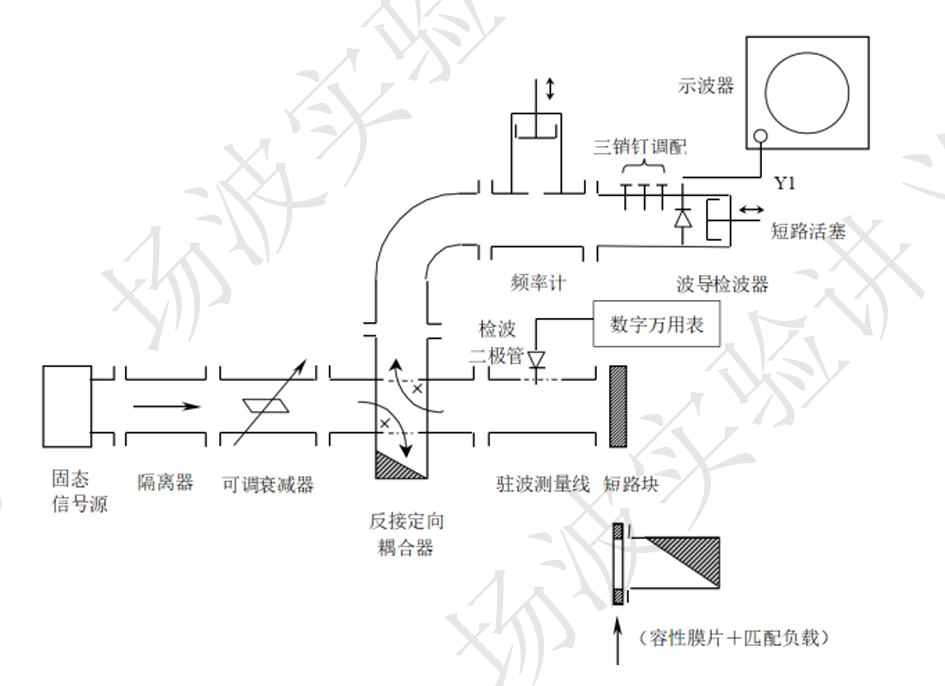
\includegraphics[width=0.75\linewidth]{figures/device.png} % 数字表示放缩比例
    \caption{波导测量系统}
\end{figure}

\section{实验内容}
建立实验装置：

把各部件连按成图1所示测量系统。注意十字孔定向耦合器的连接方向， 在本系统中定向耦合器连接方向为对反射功率采样。(定向耦合器从主波导耦合到副波导的功率传输规律是：功率传输方向通过两个耦合孔的连线拐弯，见图1中标识)。实验开始前可调衰减器保持一定衰减量。

驻波测量线探针插入深度为 0 驻波测量线输出电缆连接到高精度数字万用表输入口，万用表选择 AC 电压测最模式(测最检波信号的有效值)。波导检波器输出电缆接到示波器 CH1 输入口，并把示波器输入选择置于直流工作状态。

\subsection{工作频率f测量}
(1)测量线开口端用短路块短接。

(2)接通固态微波信号源，工作状态选择方波调制。

(3)调节波导检波器中的短路活塞或三销钉调配器使示波器上显示的检波输出(方波)幅度最大。如果示波器上显示的输出幅度还不够大，可适当减少可调衰减器的衰减量，反之增加可调衰减器的衰减量。(注意：由于微波频率高，波长短，故调节时必须如同调节显微镜一样细心，而且在用三销钉调节时，销钉插入深度不能超过波导高度$b$的一半，否则会产生全反射以至无信号检出。)

(4)用直读式频率计测量此时系统的工作频率$f$ (注意：调节时必须缓慢细调，由于频率计等效于电路中的一个并联谐振回路，当它产生谐振时，一部份能量被吸收，相应地串接在后面的检波器得到的能量就变小，于是示波器上看到的方波幅度也就变小，因而调节时注意观察示波器上的方波幅度，当看到幅度有突变，且变得最小时，频率计上读得的读数就是微波信号源的振荡频率，单位为GHz。频率计的读法是：两条水平红线夹着的那一行刻度线与垂直红线相交的



\subsection{波导波长测量}

(1)先调节测量线探针插入深度为 lmm 左右，再细心调节测量线上的检波调配装置，使数字万用表上指示的检波输出信号最大，即检波匹配(注意：为使测量线的检波二极管工作在小信号的平方率检波区，探针插入深度不能太深，否则探针本身会引起较大反射，使测量数值产生较大误差)。沿波导横向移动驻波测量探针，使探针位于驻波波腹点(检波的输出最大),此时再调节衰减器使数字万用表读数为0.500mV(设定信号在合适的大小),记录此时衰减器的刻度， 以便之后测量。

(2)慢慢地横向移动测量线探针，记下相邻两个驻波波节点的位置$d_{min1}$、$d_{min2}$的刻度值。

\subsection{容性膜片等效负载的测量}

实验装置仍如图1。实验步骤如下：

(1)测量线开口端接短路块，横向移动测量线探针，找到一个驻波波节点位置$d_{min1\text{(短)}}$并作记录(即等效短路面位置)

(2)拆下短路块，接上容性膜片和匹配负载,从$d_{min1\text{(短)}}$ 位置往振荡源信号方向移动驻波测量线探针位置，测得第一个驻波最小点位置$d_{min1\text{(膜片)}}$,并作记录。

(3)测量此时的驻波系数，即横向移动驻波测量线探针位置，在数字万用表上读出检波输出最大值 $P_{max}$与最小值$P_{min}$(注意：考虑到检波器为小信号平方率检波，故数字万用表读出的数值应为相对功率值)。

\subsection{阻抗匹配测量}
在测量线与容性膜片+匹配负载之间串接一只单销钉调配器。单销钉调配器是一个其销钉插入波导深度和纵向位置都可以调节的器件。

(1)调节衰减器衰减量，使示波器有足够的方波信号显示。

(2)细心调节销钉调配器销钉的横向位置和插入波导的深度，使示波器上显示的信号最小(最好能到零)。进而提高示波器的灵敏度和增加输入功率，重复上一调节过程直到当示波器的灵敏度为最高和输入功率为最大且又在示波器上观察到的信号为最小为止，即找到最佳匹配位置

(3)适当增加可调衰减器的衰减量之后，横向移动驻波测量线，记录该输入功率下数字万用表上的$P_{max\text{(匹配 1)}}$与$P_{min\text{(匹配 2)}}$ ,并计算此时的驻波系数$\rho$。

$\text{负载端直接接入匹配负载,横向移动驻波测量线,记录该输入功率下数字万用表上的}\\P_{max\text{(匹配 2)}}\text{与}P_{min\text{(匹配 2)}}\text{,并计算此时的驻波系数}\rho\text{匹配。}$

\section{实验结果和数据记录}
\subsection{工作频率f测量}

\begin{figure}[H]
    \centering
    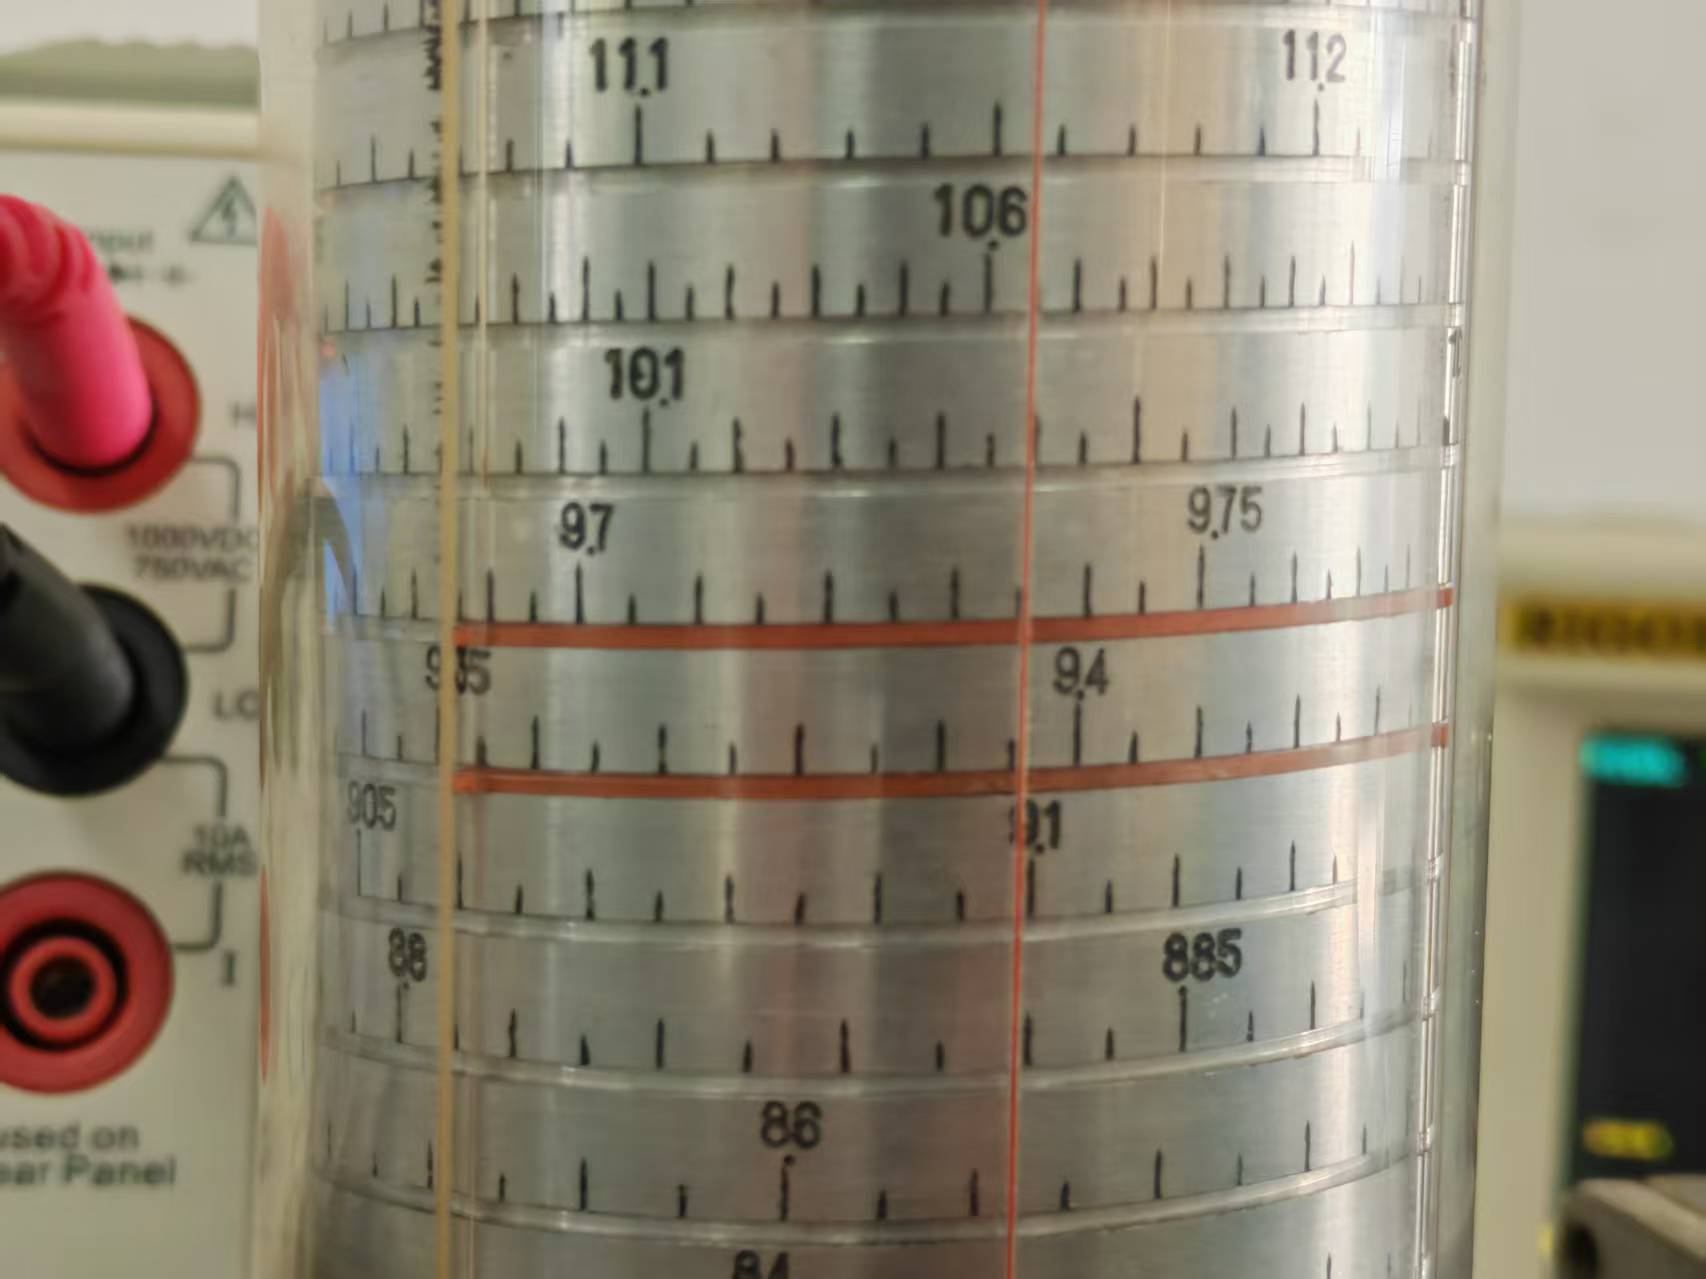
\includegraphics[width=0.3\linewidth]{figures/p11.jpg} % 数字表示放缩比例
    \caption{工作频率f读数}
\end{figure}

如图工作频率f测量值为：9.396GHz

\subsection{波导波长测量}

\begin{figure}[H]
    \centering
    \begin{minipage}{.33\textwidth}
        \centering
        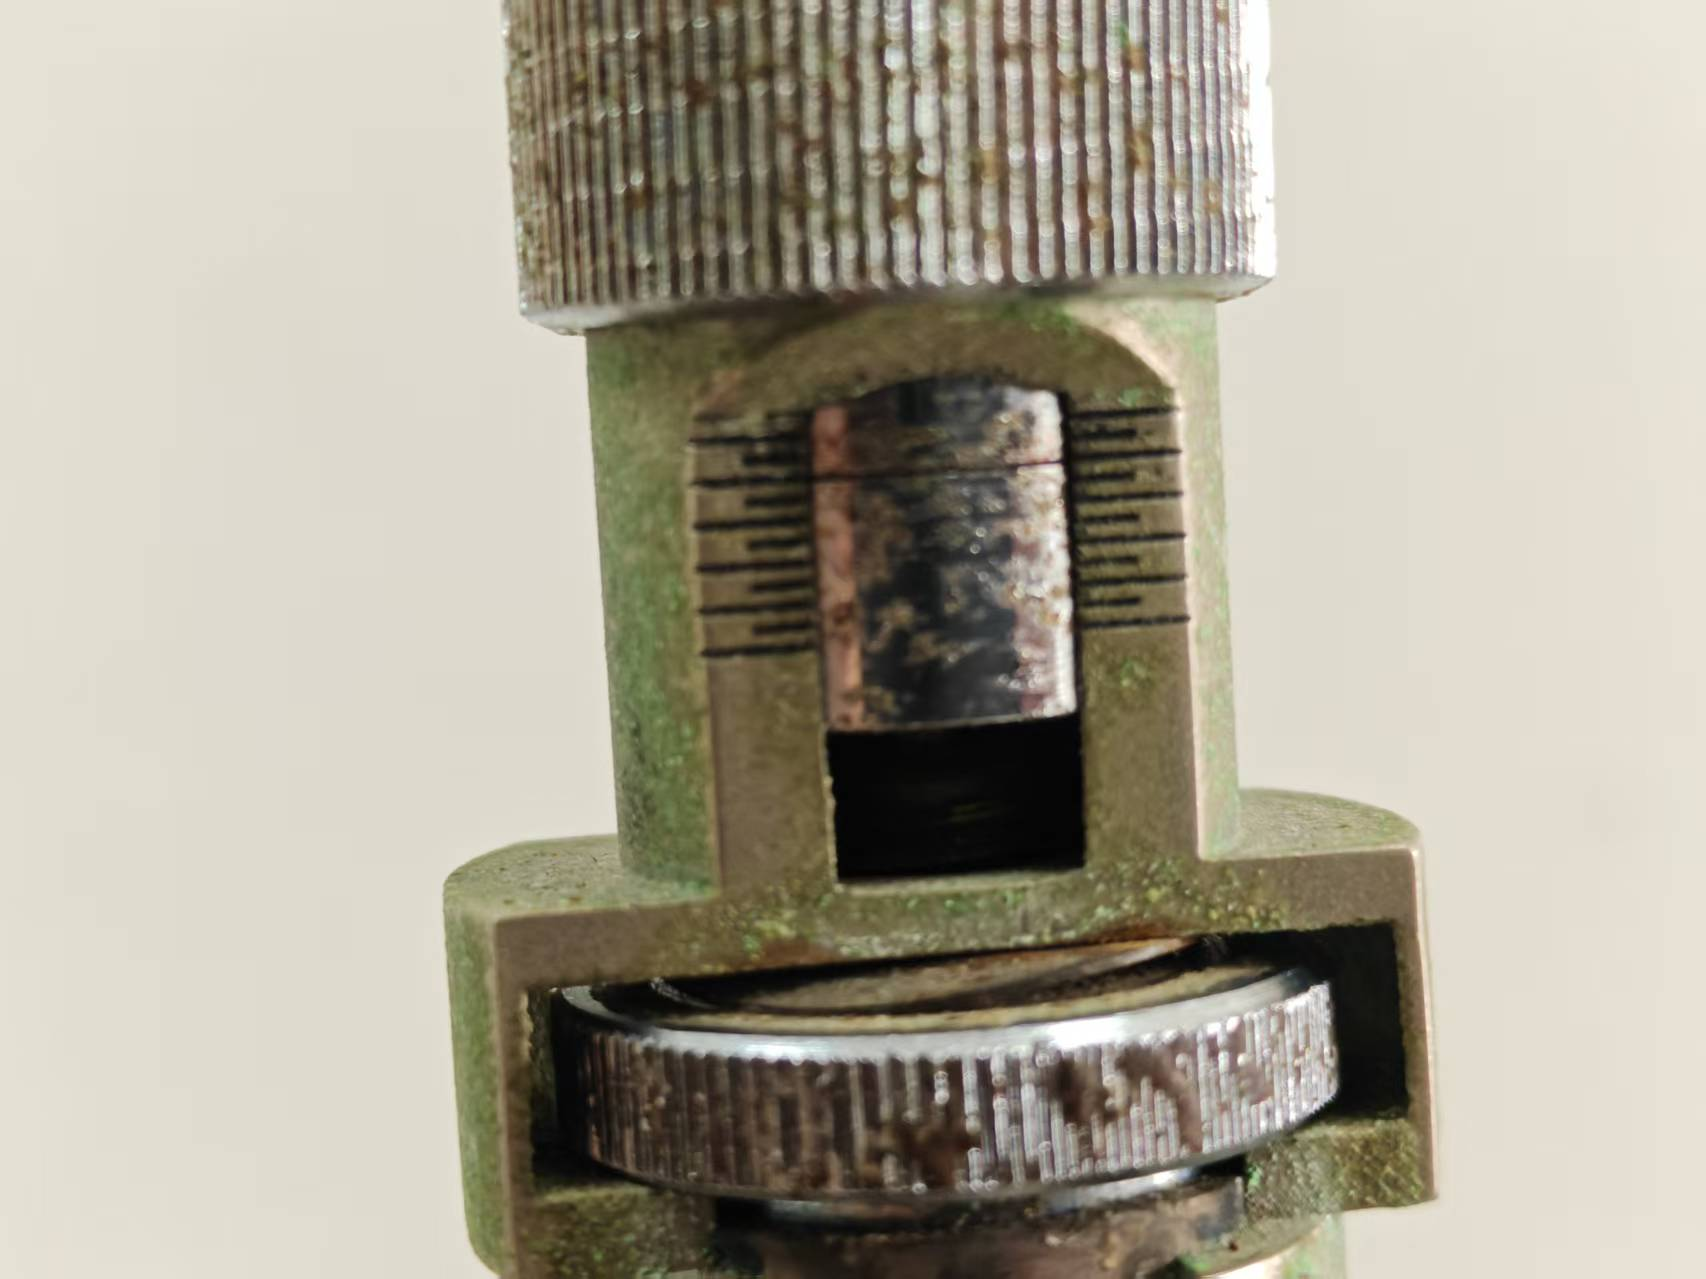
\includegraphics[width=.95\linewidth]{figures/p12.jpg}
        \caption{探针插入1mm}
        \label{fig:probe-insertion}
    \end{minipage}%
    \begin{minipage}{.33\textwidth}
        \centering
        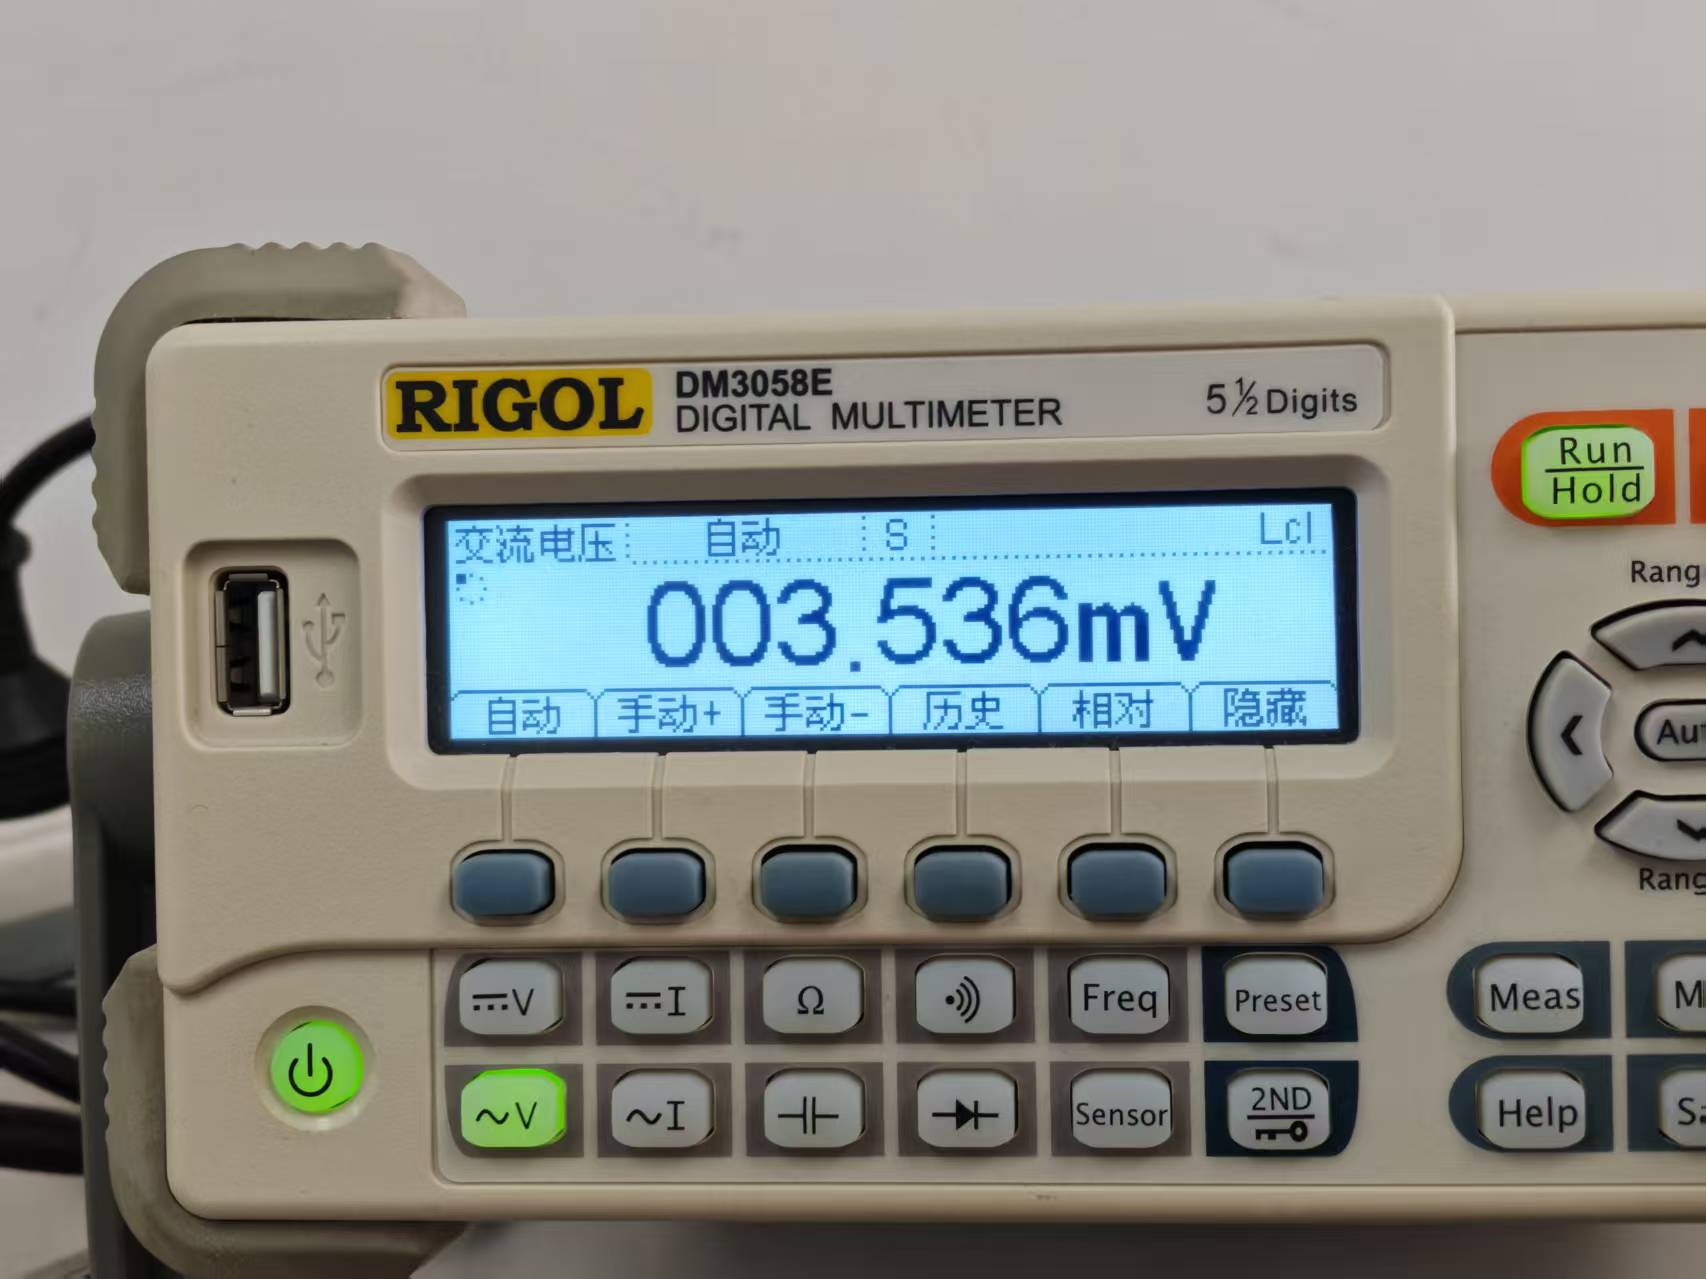
\includegraphics[width=.95\linewidth]{figures/p13.jpg}
        \caption{找到波腹}
        \label{fig:find-belly}
    \end{minipage}%
    \begin{minipage}{.33\textwidth}
        \centering
        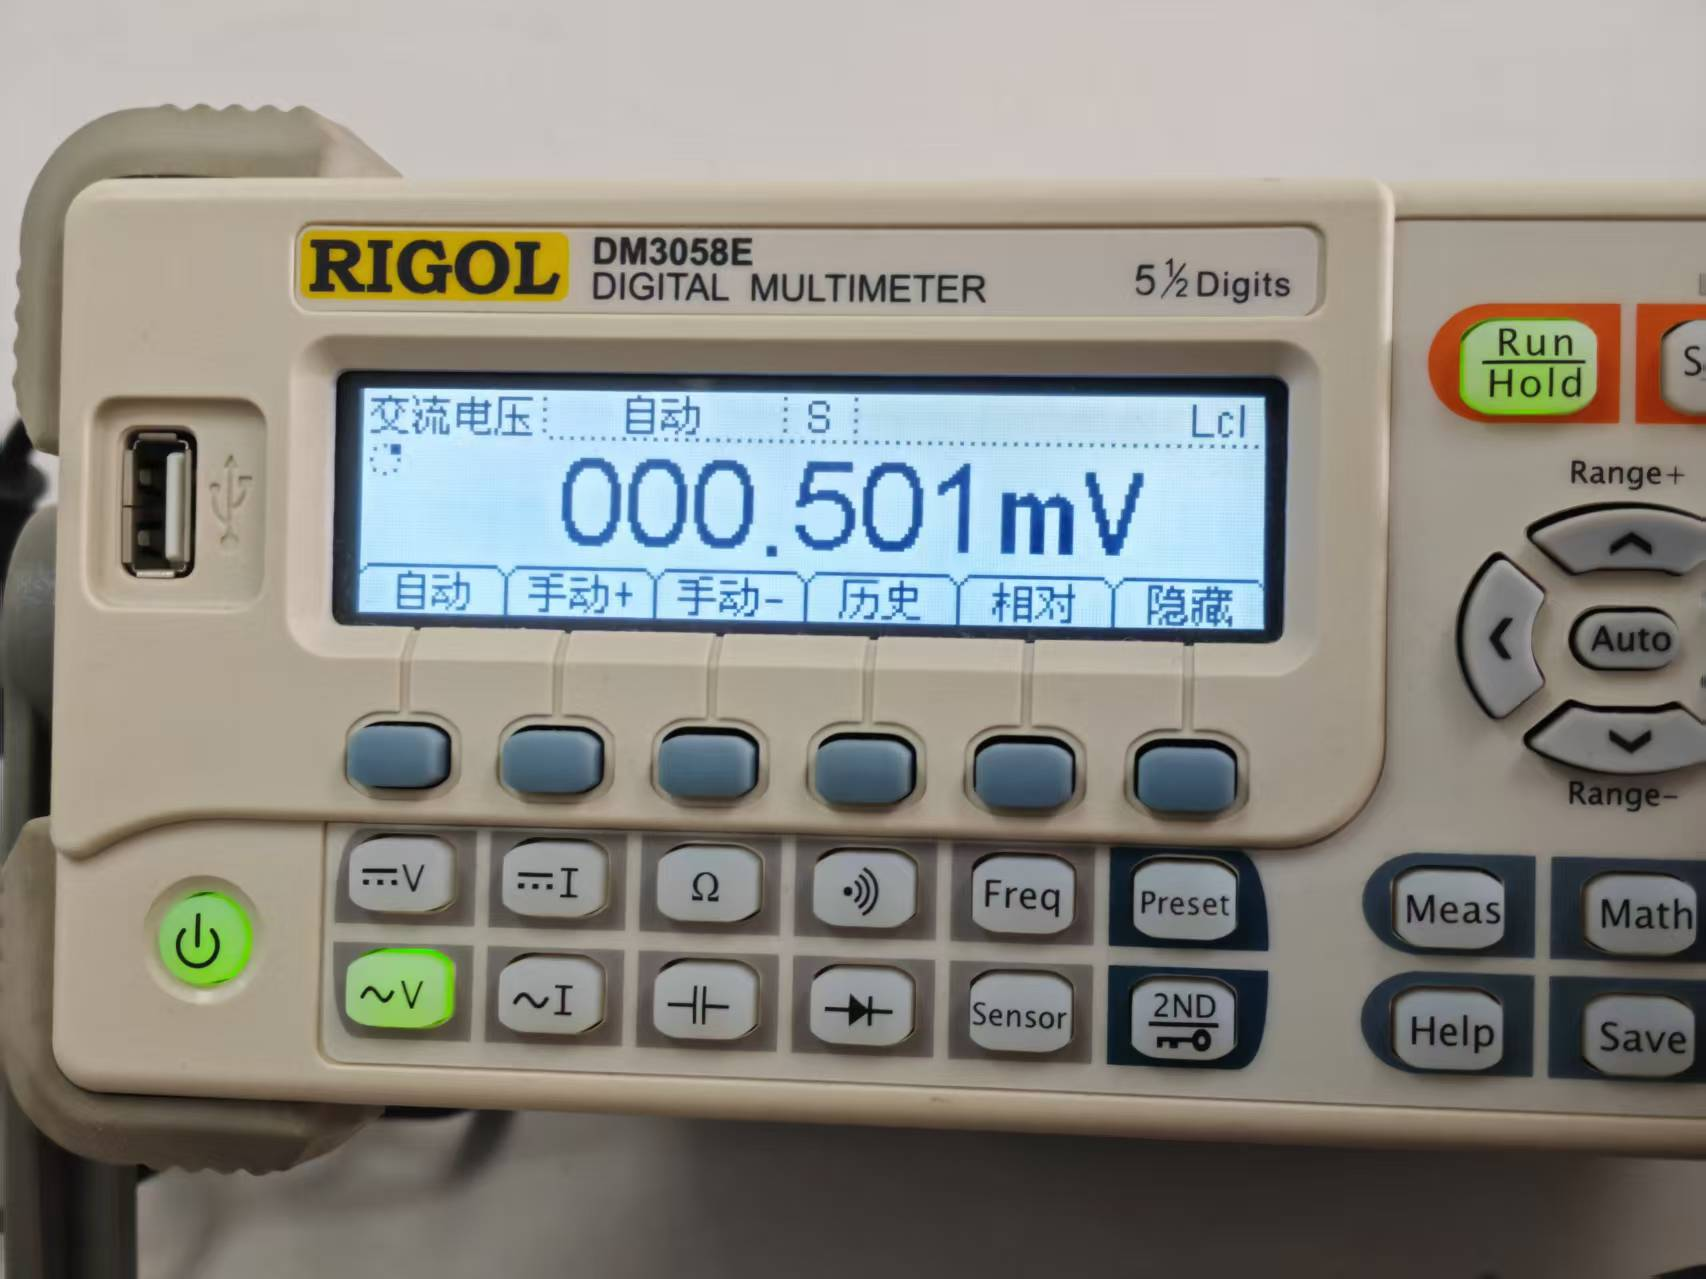
\includegraphics[width=.95\linewidth]{figures/p14.jpg}
        \caption{调节衰减器}
        \label{fig:set-signal-size}
    \end{minipage}
\end{figure}


\begin{figure}[H]
    \centering
    \begin{minipage}{.33\textwidth}
        \centering
        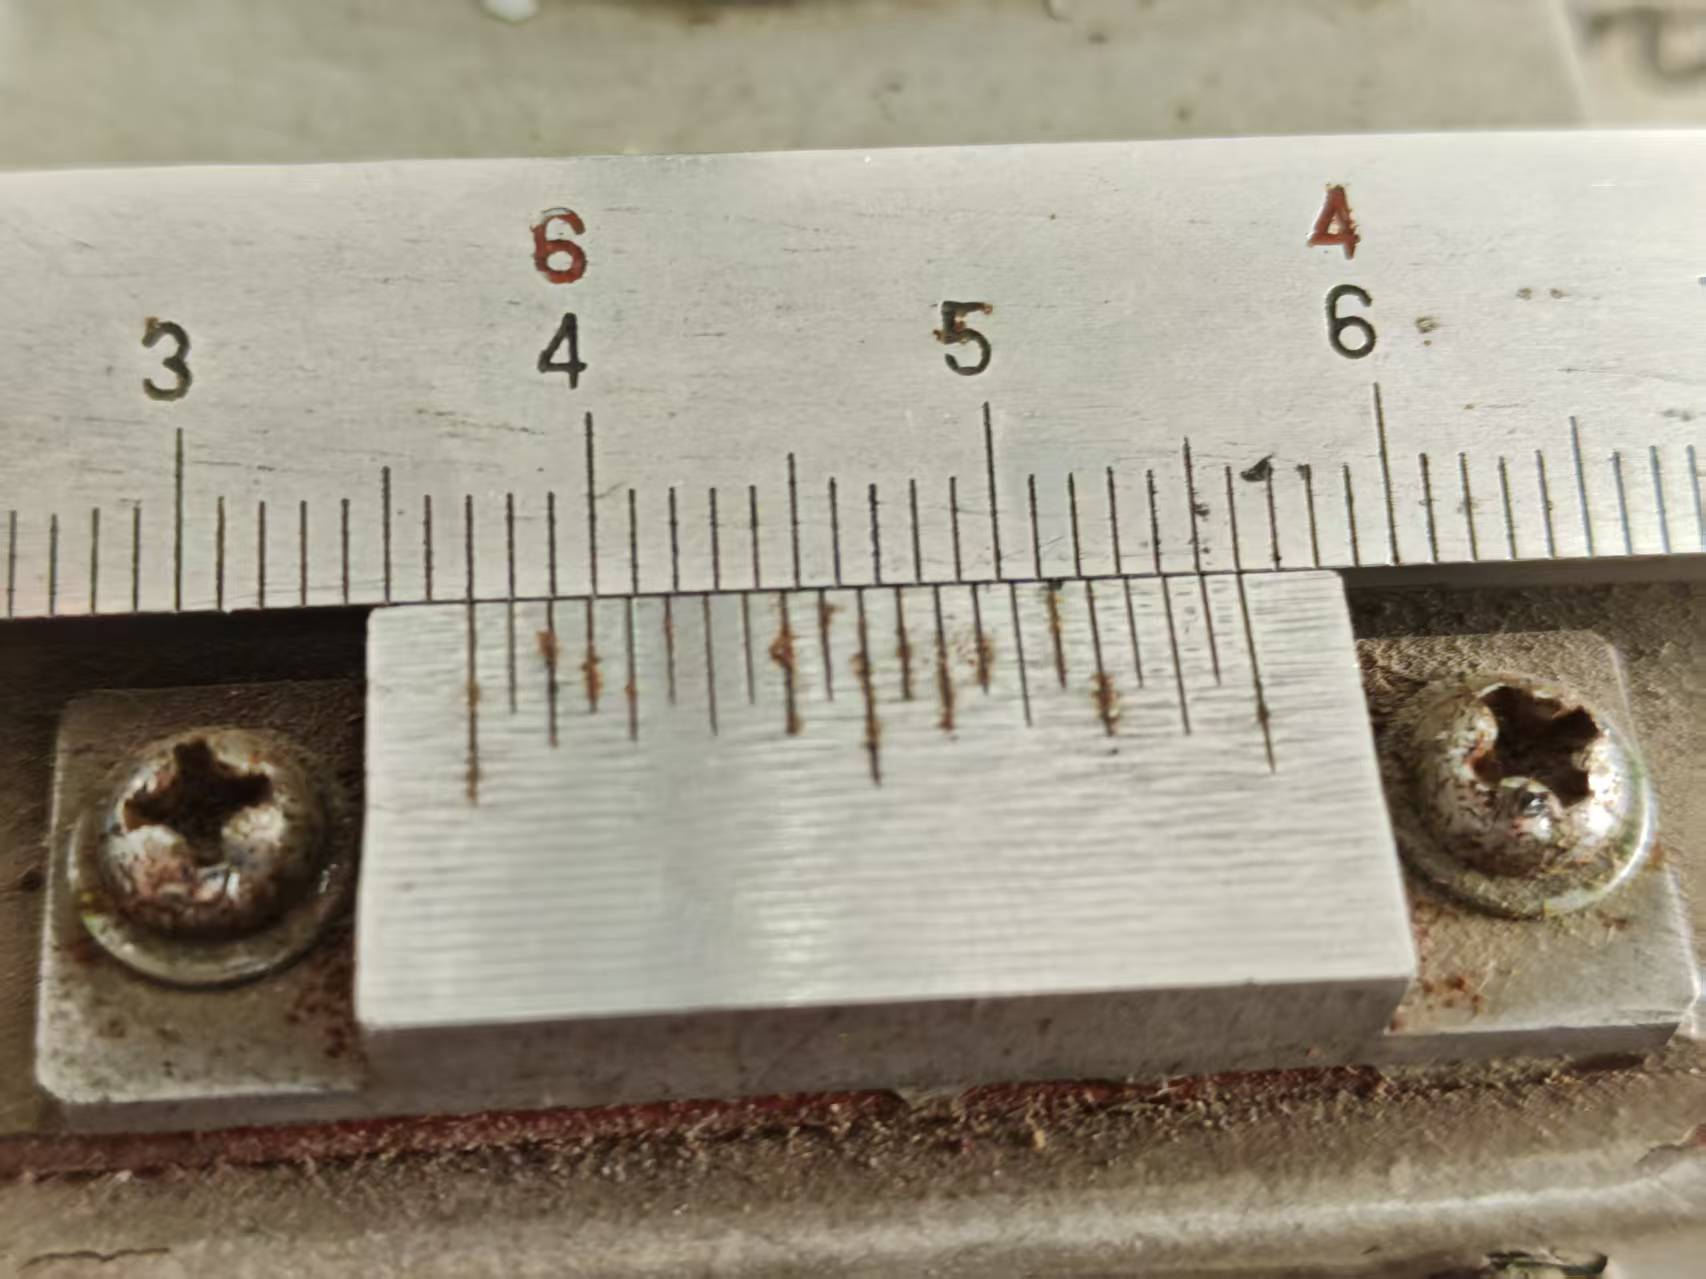
\includegraphics[width=.95\linewidth]{p21.jpg}
        \caption{dmin1}
        \label{fig:dmin1}
    \end{minipage}%
    \begin{minipage}{.33\textwidth}
        \centering
        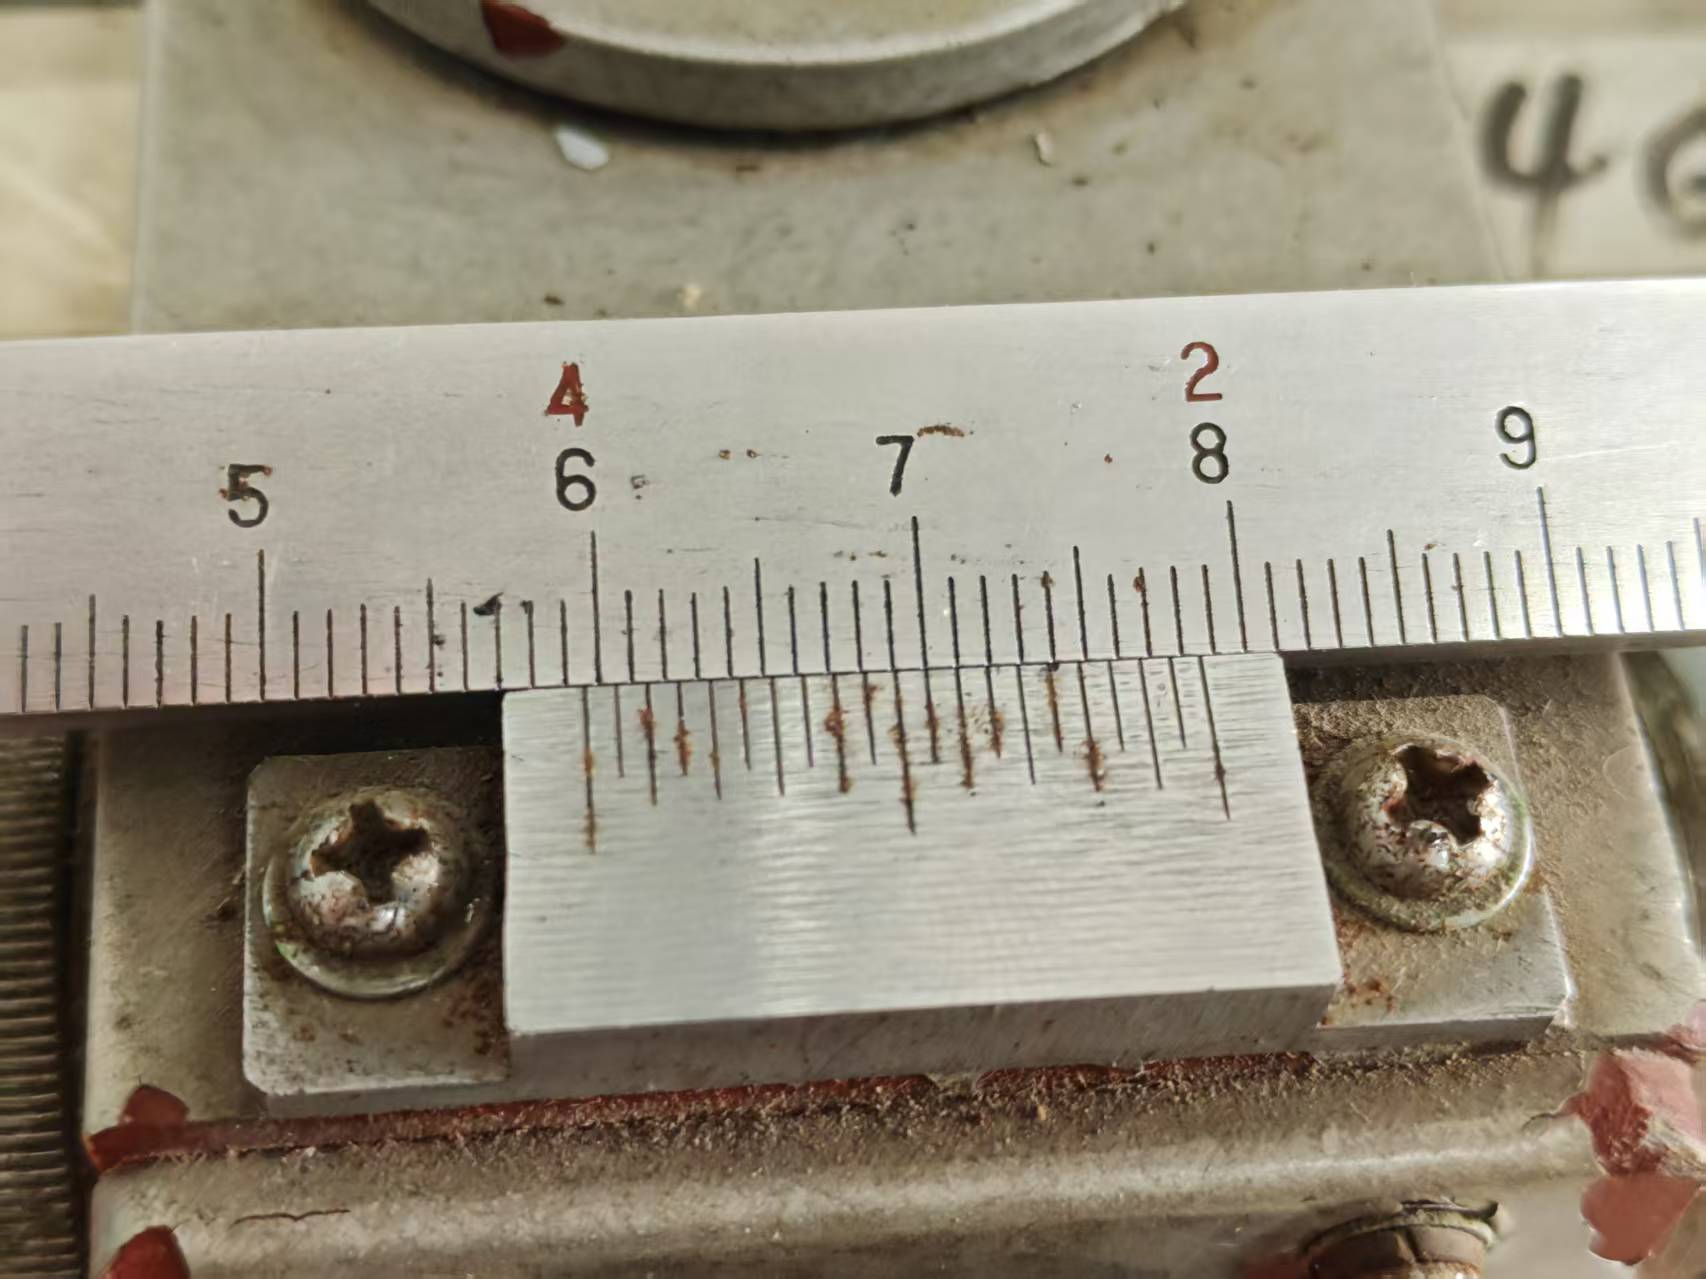
\includegraphics[width=.95\linewidth]{p22.jpg}
        \caption{dmin2}
        \label{fig:dmin2}
    \end{minipage}%
    \begin{minipage}{.33\textwidth}
        \centering
        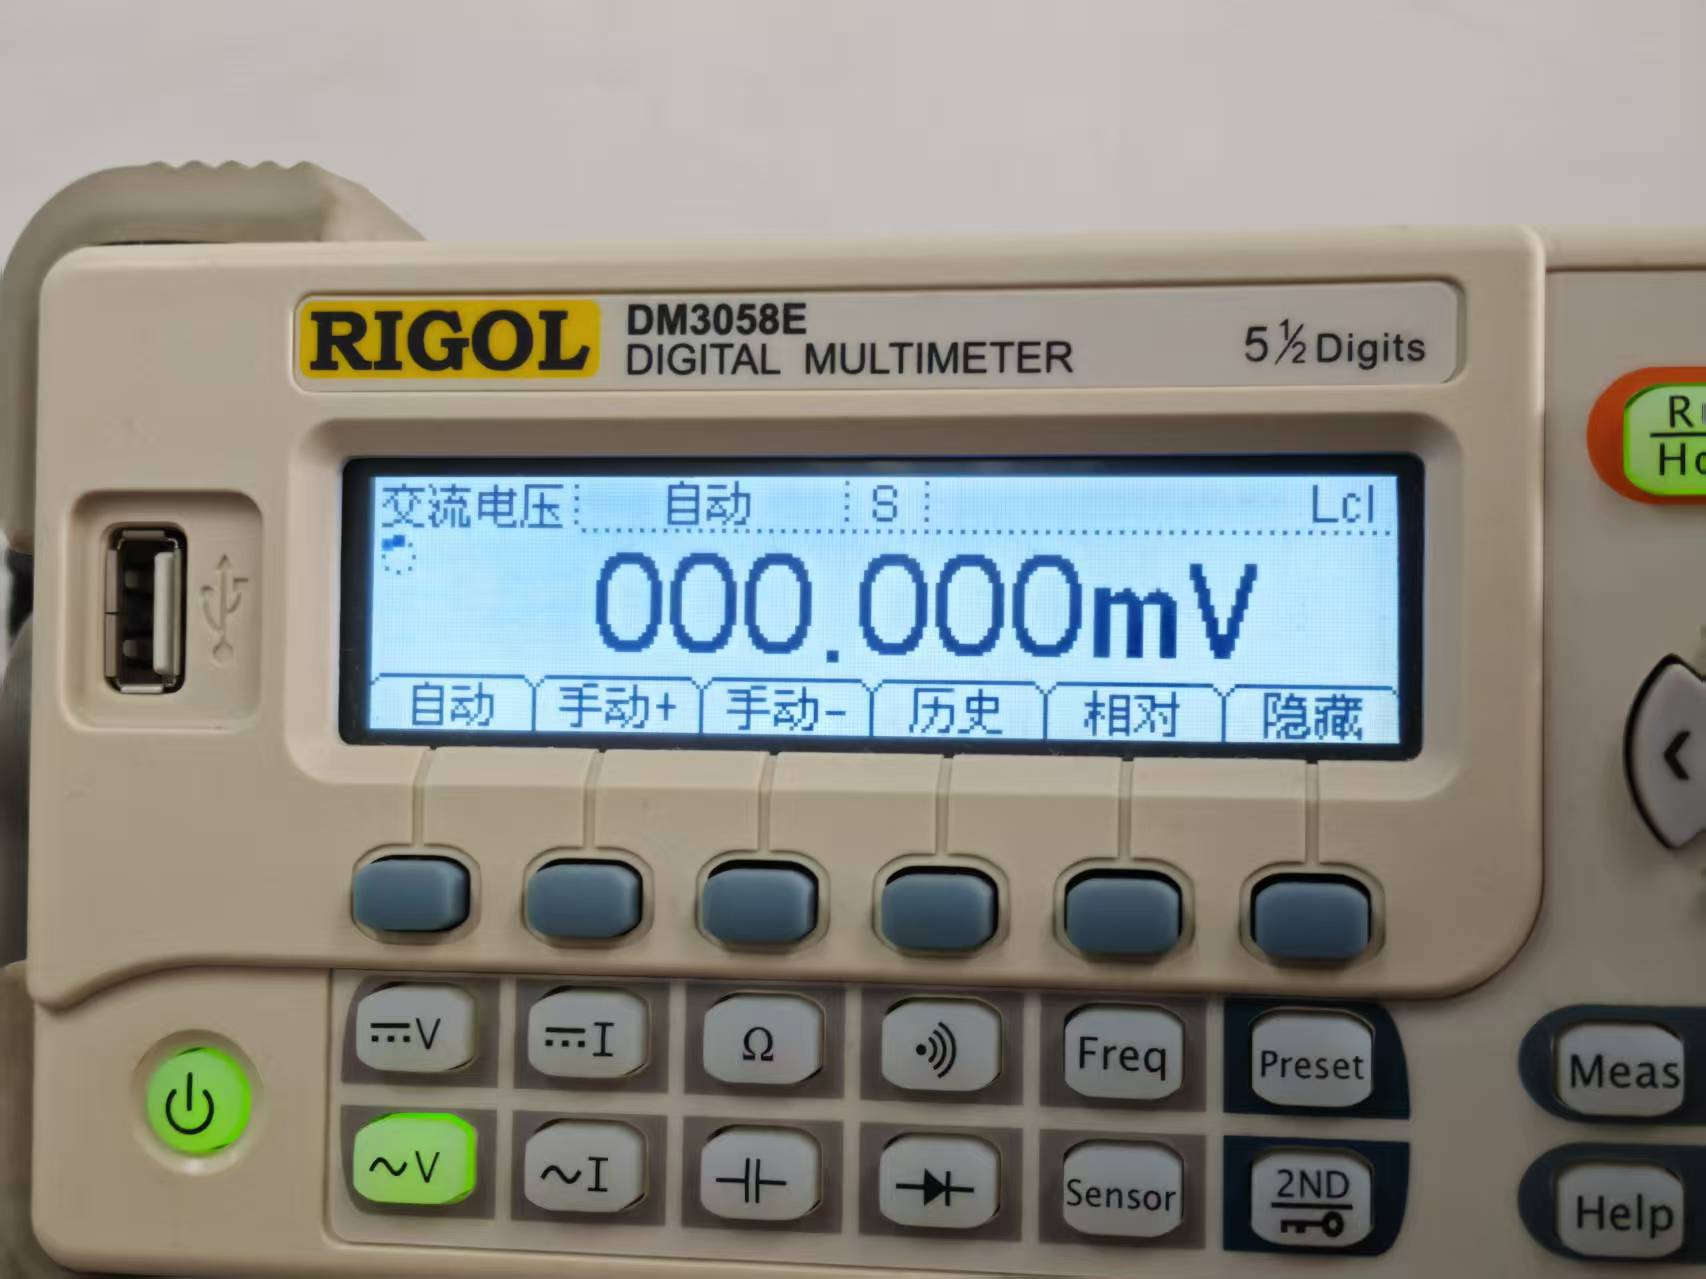
\includegraphics[width=.95\linewidth]{p23.jpg}
        \caption{波节处为0mv}
        \label{fig:0mv-image}
    \end{minipage}
\end{figure}

如图，$d_{min1}=3.700cm$、$d_{min2}=5.960cm$

【注】：此处测量时波节存在一定长度的0mV，询问老师后得知可能是由于老化缘故引起，
故通过向同一方向移动至刚到达0mV时的刻度值来测量$d_{min1}$和$d_{min2}$

\subsection{容性膜片等效负载的测量}

\begin{figure}[H]
    \centering
    \begin{minipage}{.33\textwidth}
        \centering
        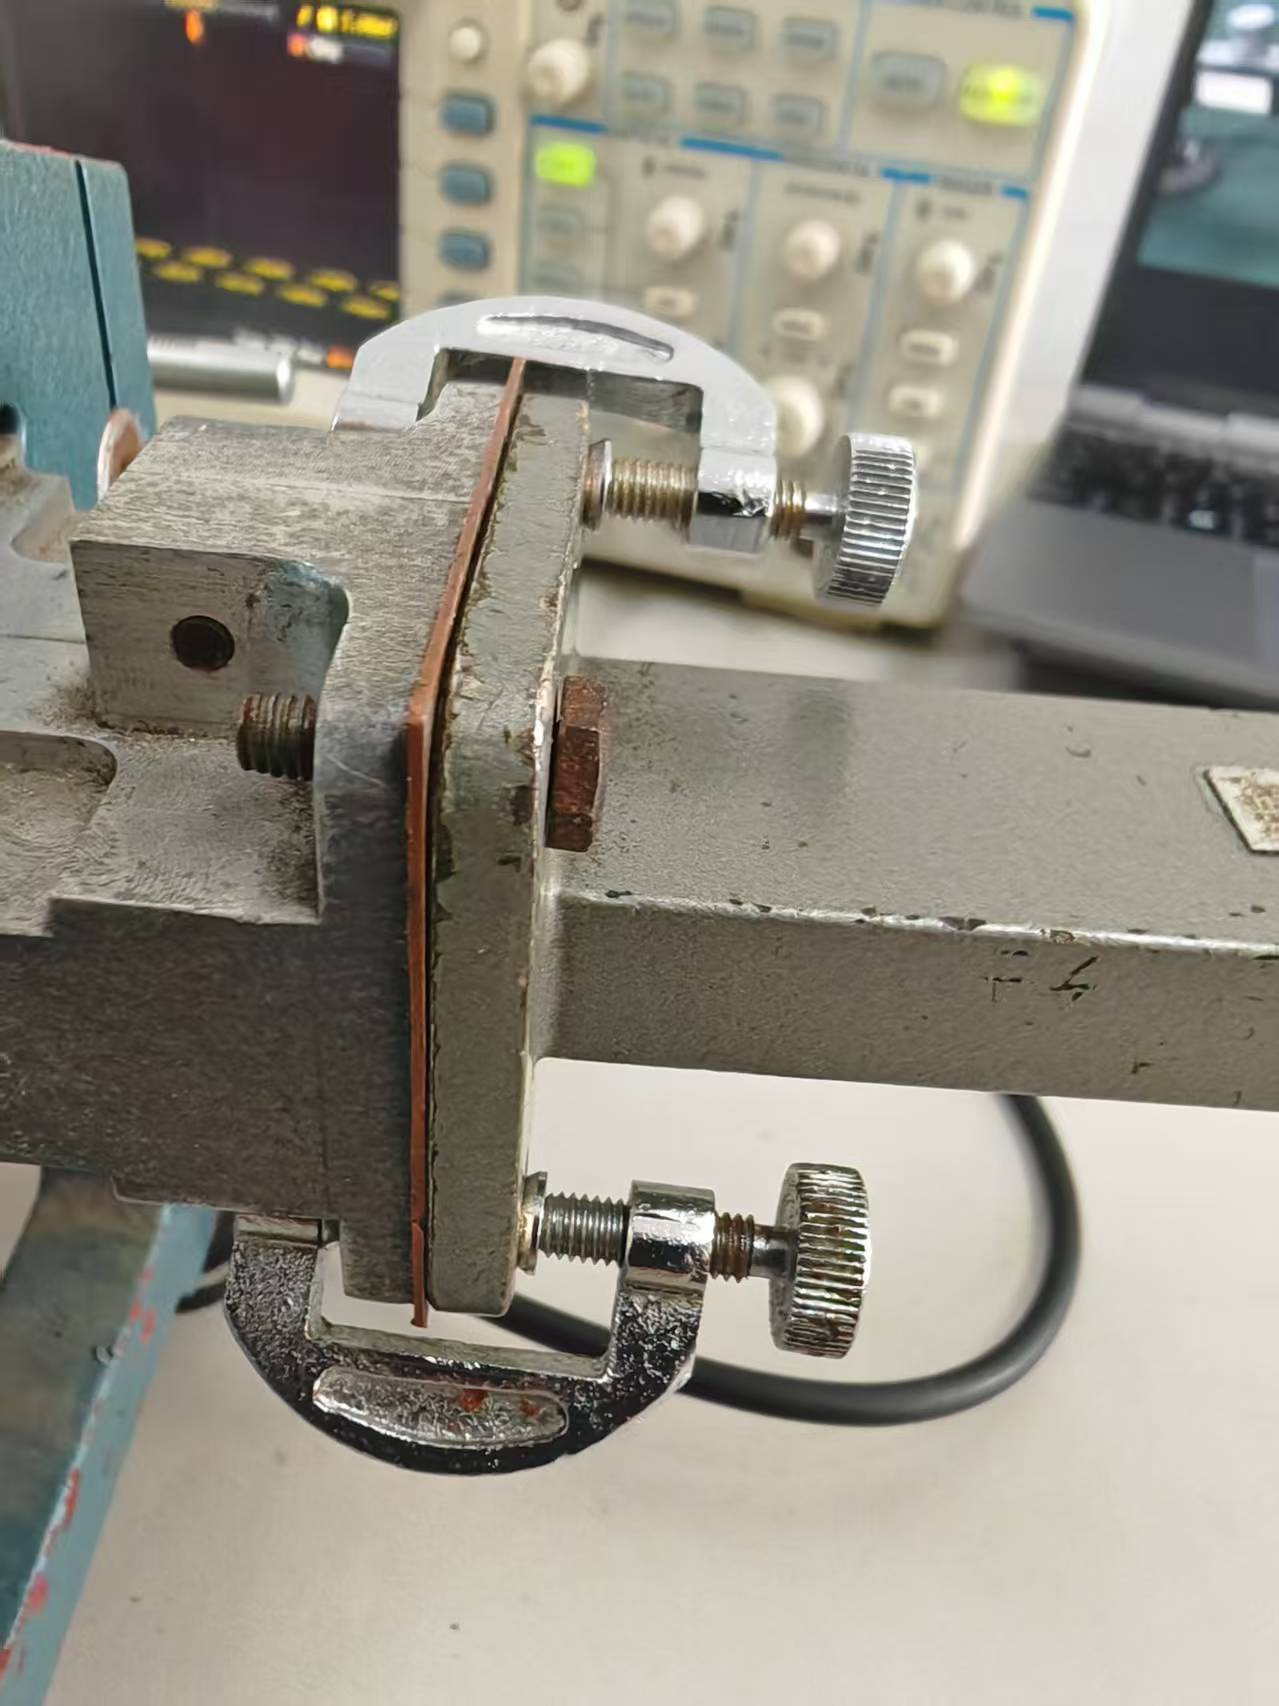
\includegraphics[width=.95\linewidth]{figures/p31.jpg}
        \caption{容性膜片接线图}
        \label{fig:0mv-image}
    \end{minipage}
    \begin{minipage}{.33\textwidth}
        \centering
        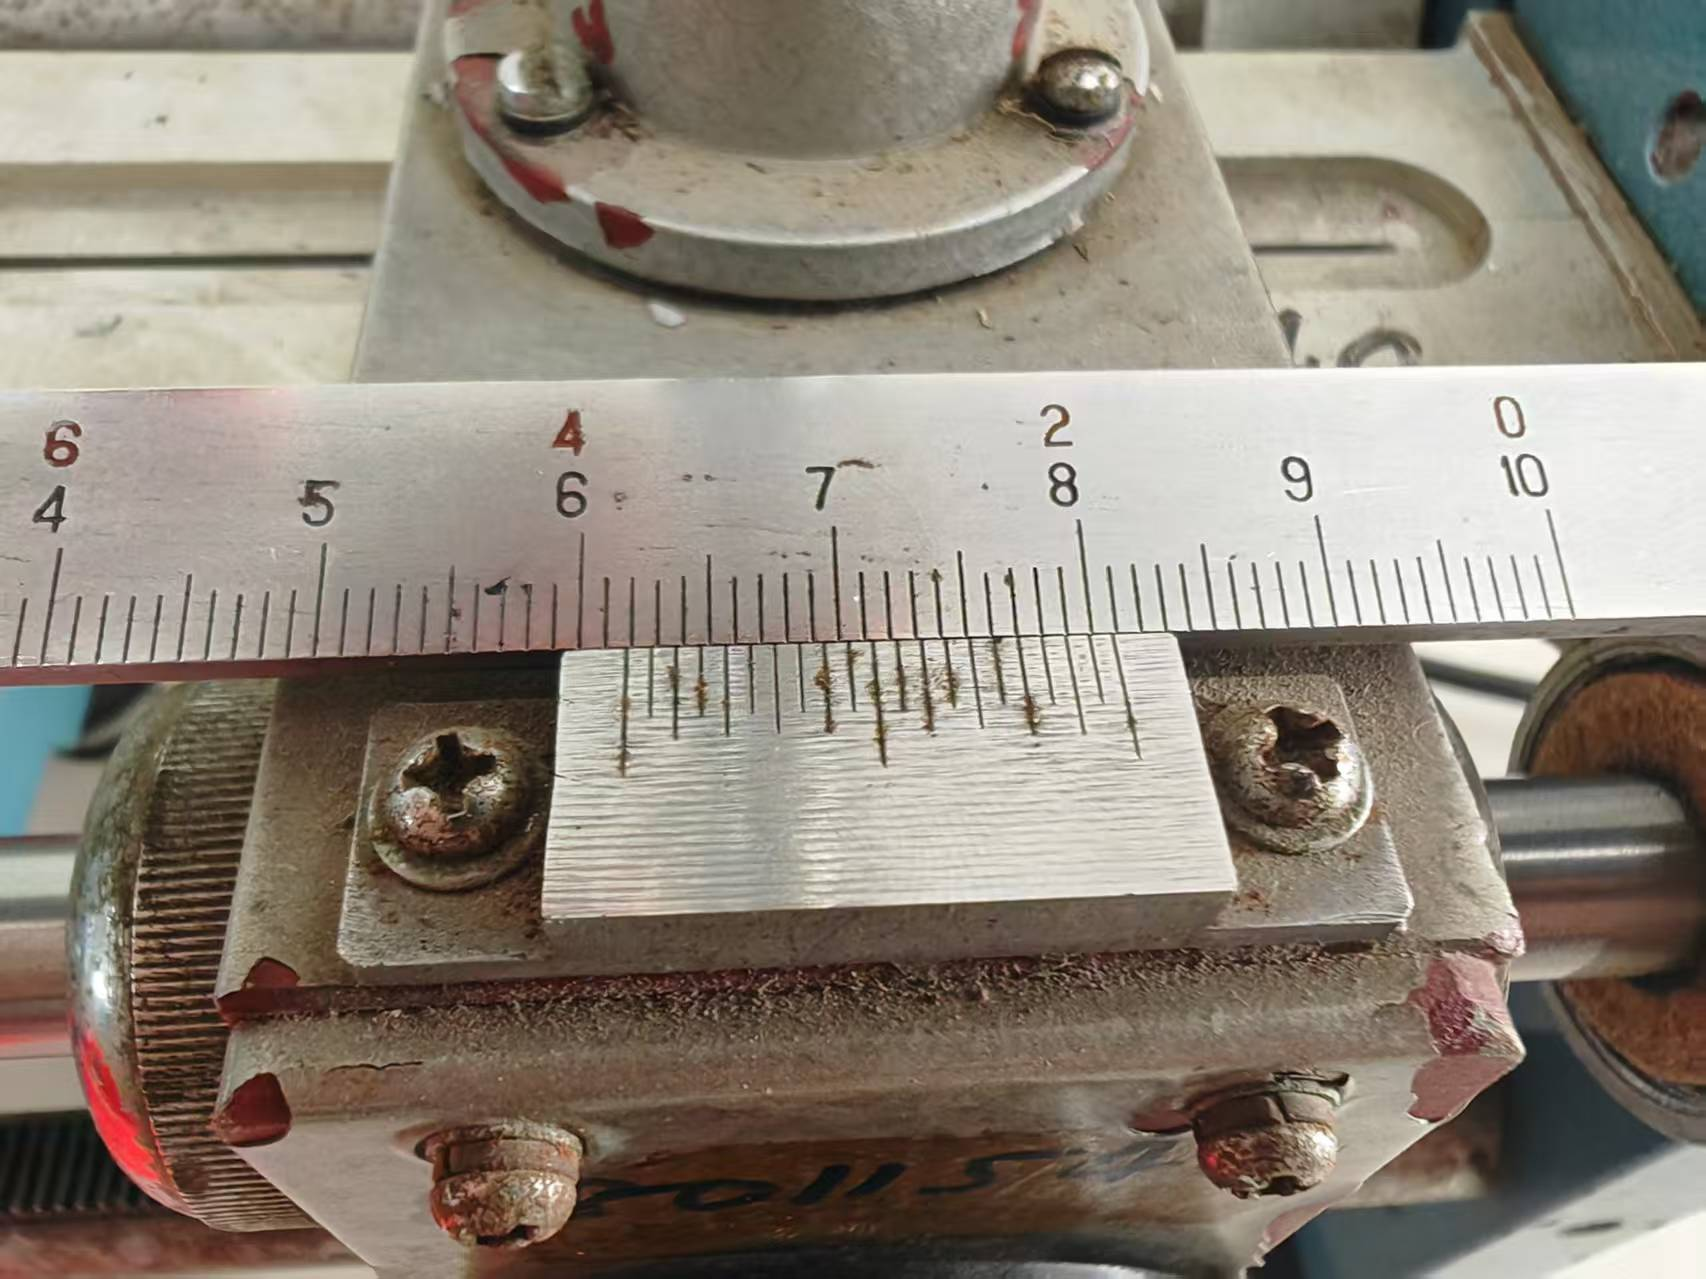
\includegraphics[width=.95\linewidth]{figures/p32.jpg}
        \caption{dmin1（短）}
        \label{fig:dmin1}
    \end{minipage}%
    \begin{minipage}{.33\textwidth}
        \centering
        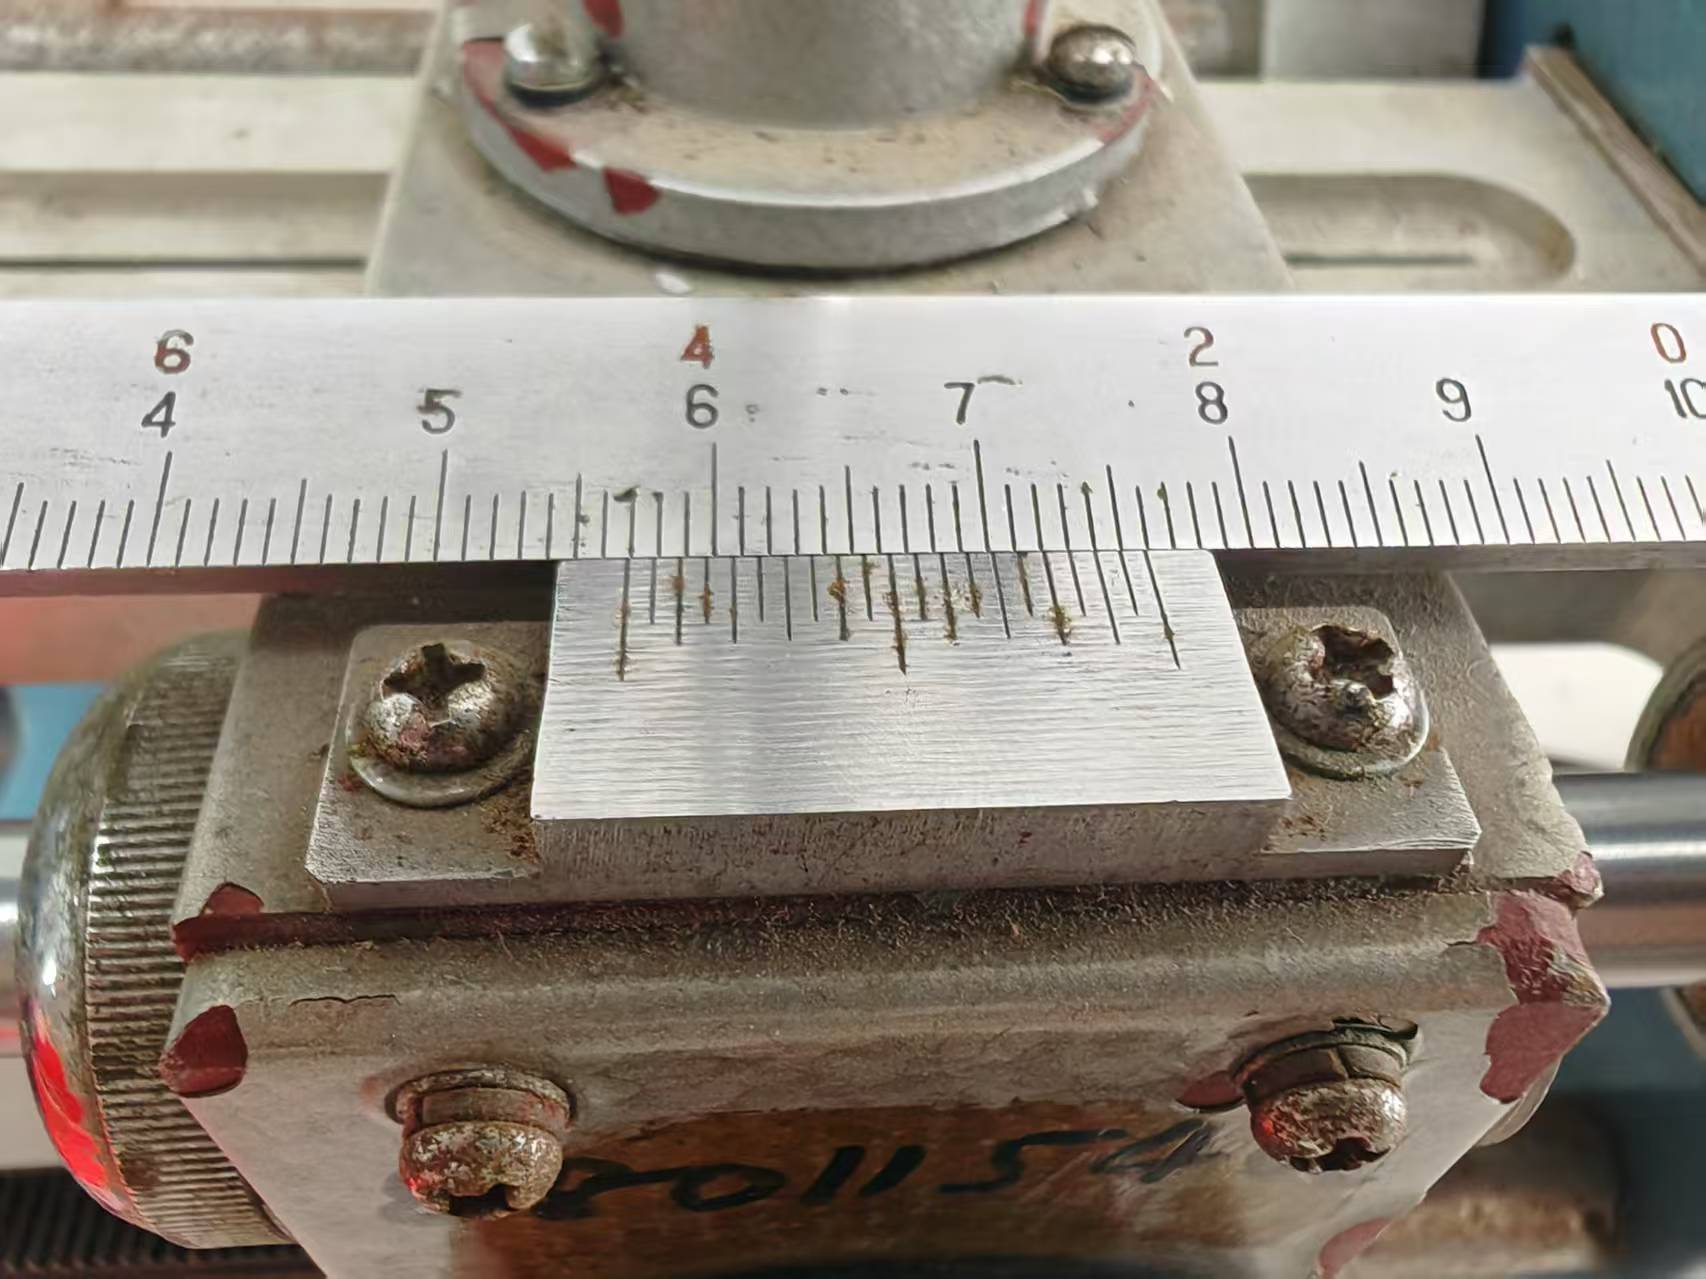
\includegraphics[width=\linewidth]{figures/p33.jpg}
        \caption{dmin1（膜片）}
        \label{fig:dmin1}
    \end{minipage}%
\end{figure}


\begin{figure}[H]
    \centering
    
    \begin{minipage}{.4\textwidth}
        \centering
        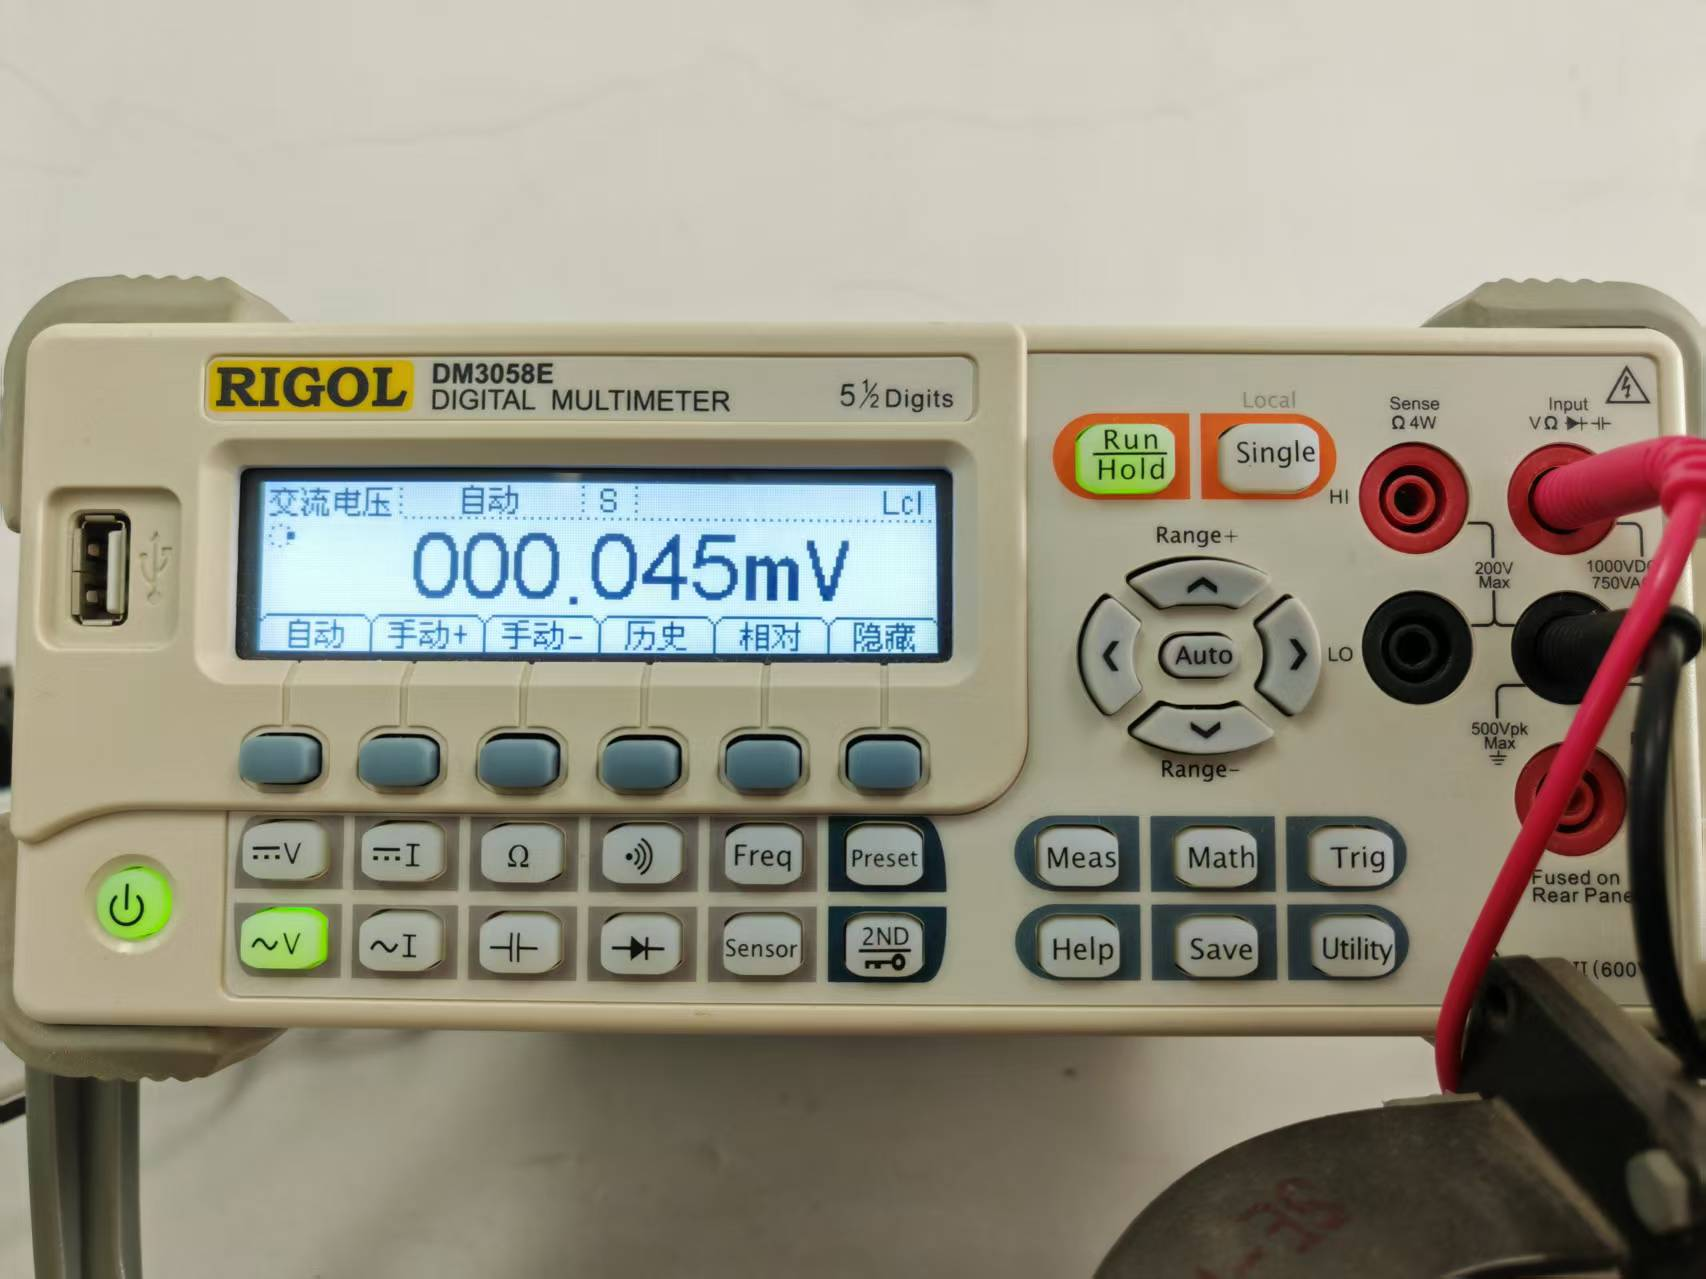
\includegraphics[width=.95\linewidth]{figures/p34.jpg}
        \caption{pmin}
        \label{fig:dmin2}
    \end{minipage}%
    \begin{minipage}{.4\textwidth}
        \centering
        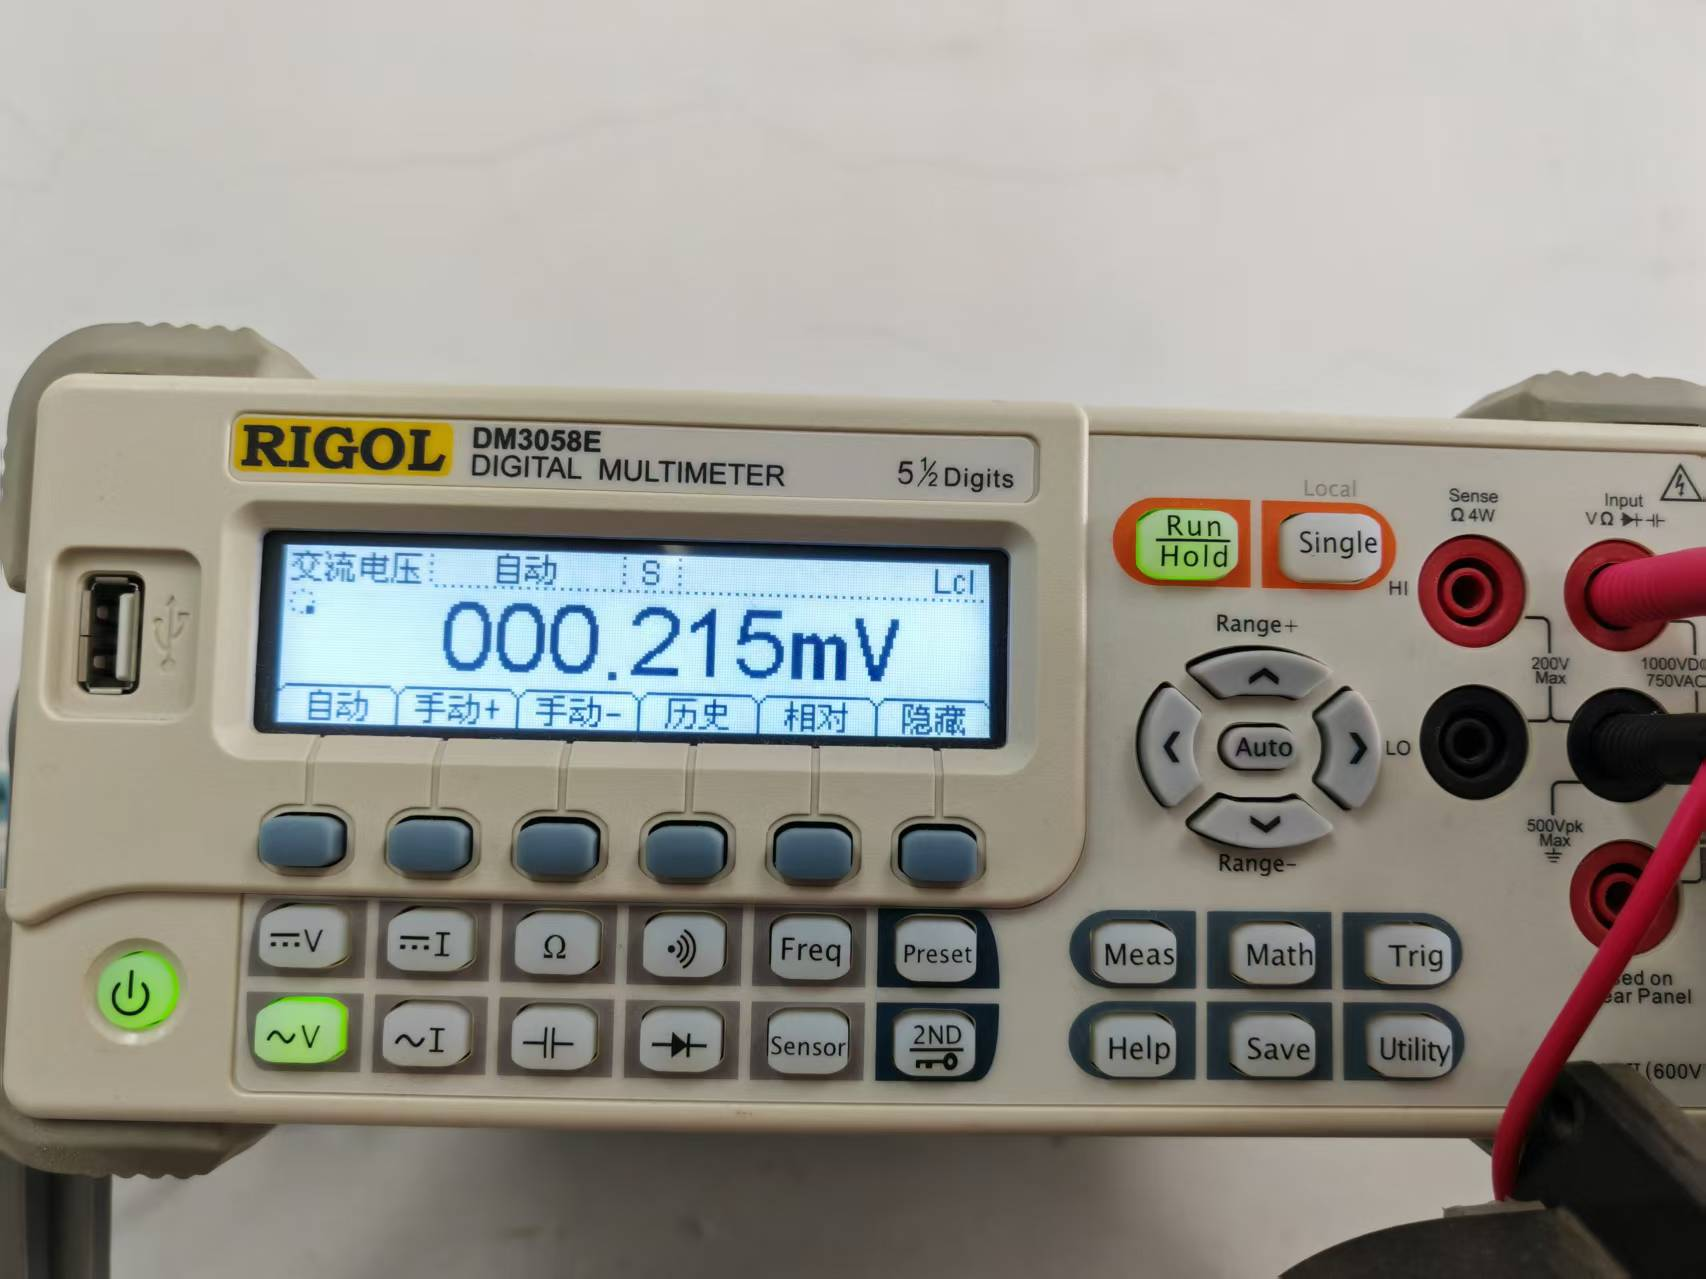
\includegraphics[width=.95\linewidth]{figures/p35.jpg}
        \caption{pmax}
        \label{fig:0mv-image}
    \end{minipage}
\end{figure}

如图，测量线开口接短路块，测得第一个驻波波节点位置$d_{min1\text{(短)}}=6.180cm$
    
测量线接容性膜片+匹配负载，测得第一个驻波波节点位置$d_{min1\text{(膜片)}}=5.685cm$

检波输出相对功率最小值$P_{min}=0.045mV$

输出相对功率最大值$P_{max}=0.215mV$

\subsection{阻抗匹配测量}

\begin{figure}[H]
    \centering
    \begin{minipage}{.24\textwidth}
        \centering
        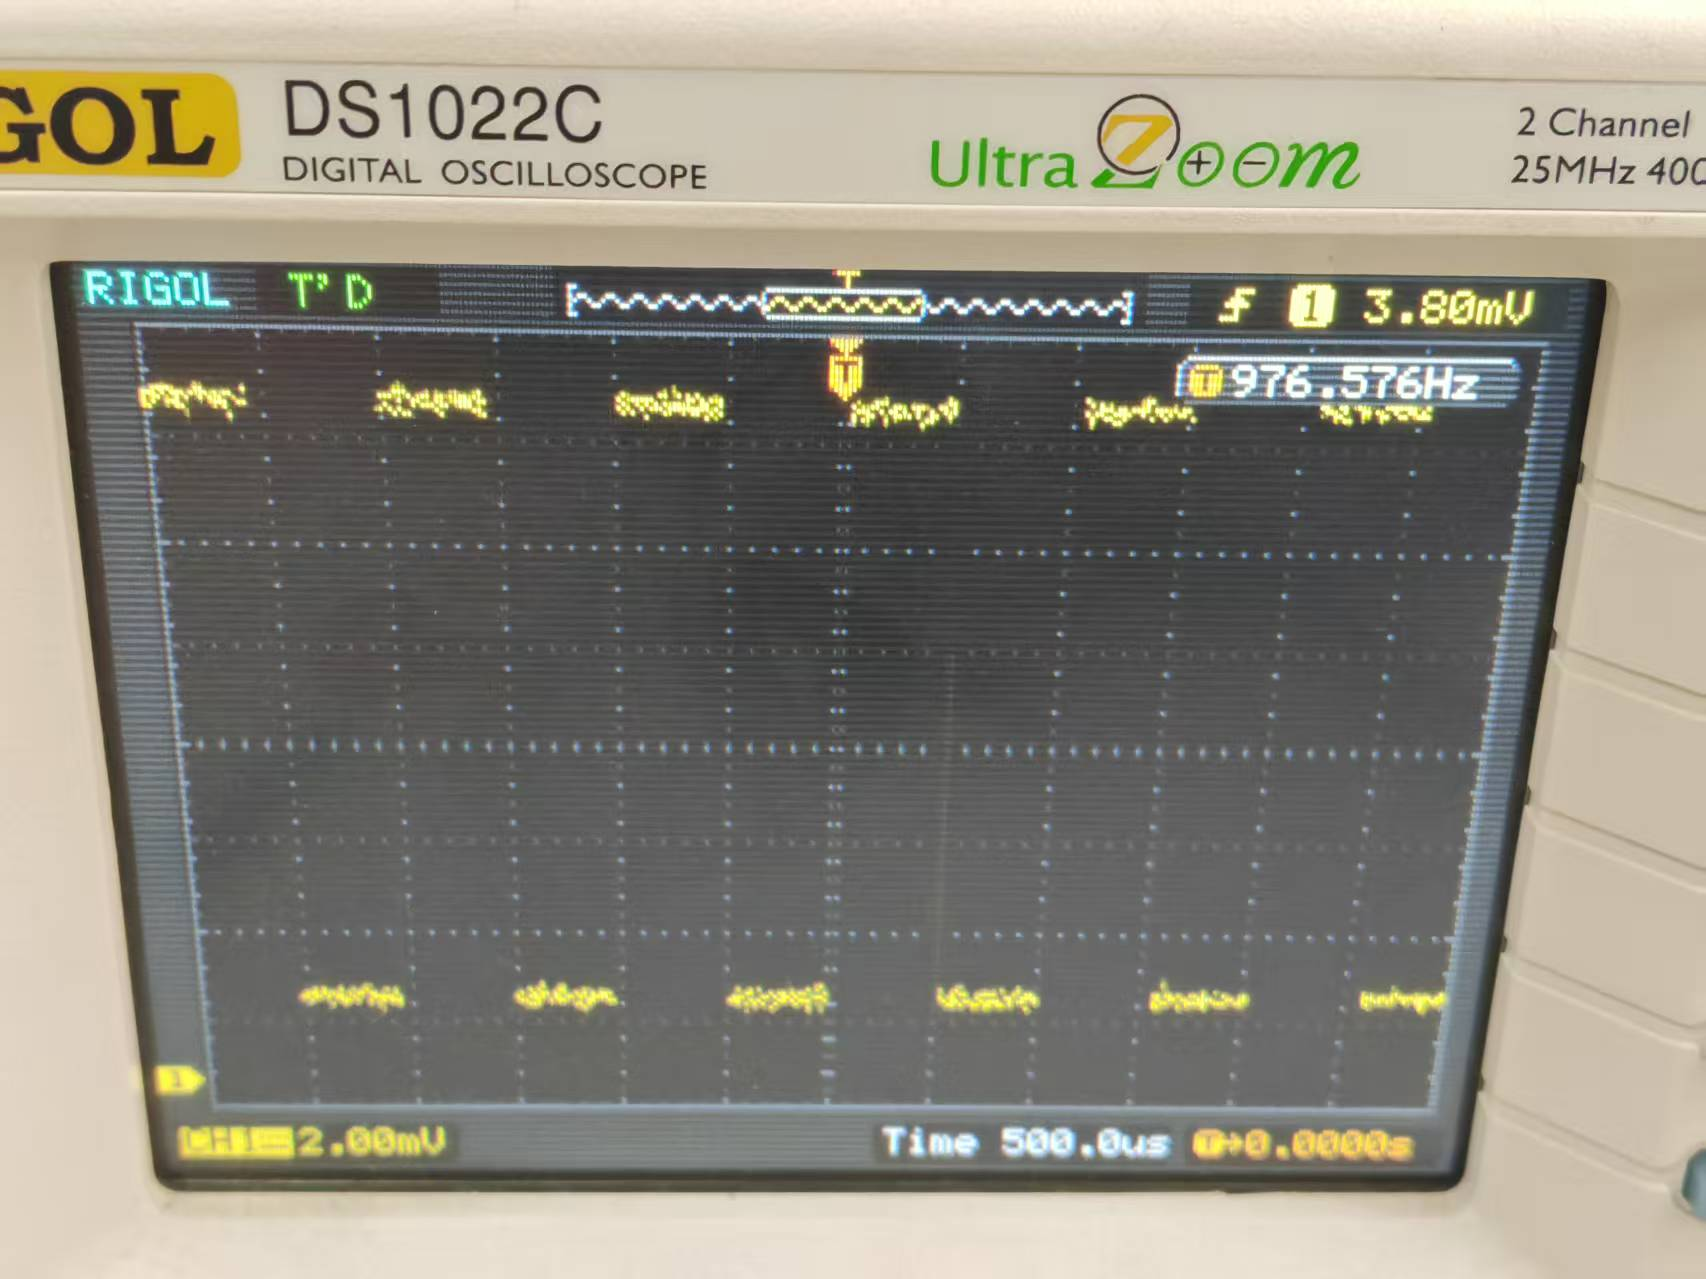
\includegraphics[width=.95\linewidth]{figures/p41.jpg}
        \caption{调节衰减}
        \label{fig:assembly}
    \end{minipage}%
    \begin{minipage}{.24\textwidth}
        \centering
        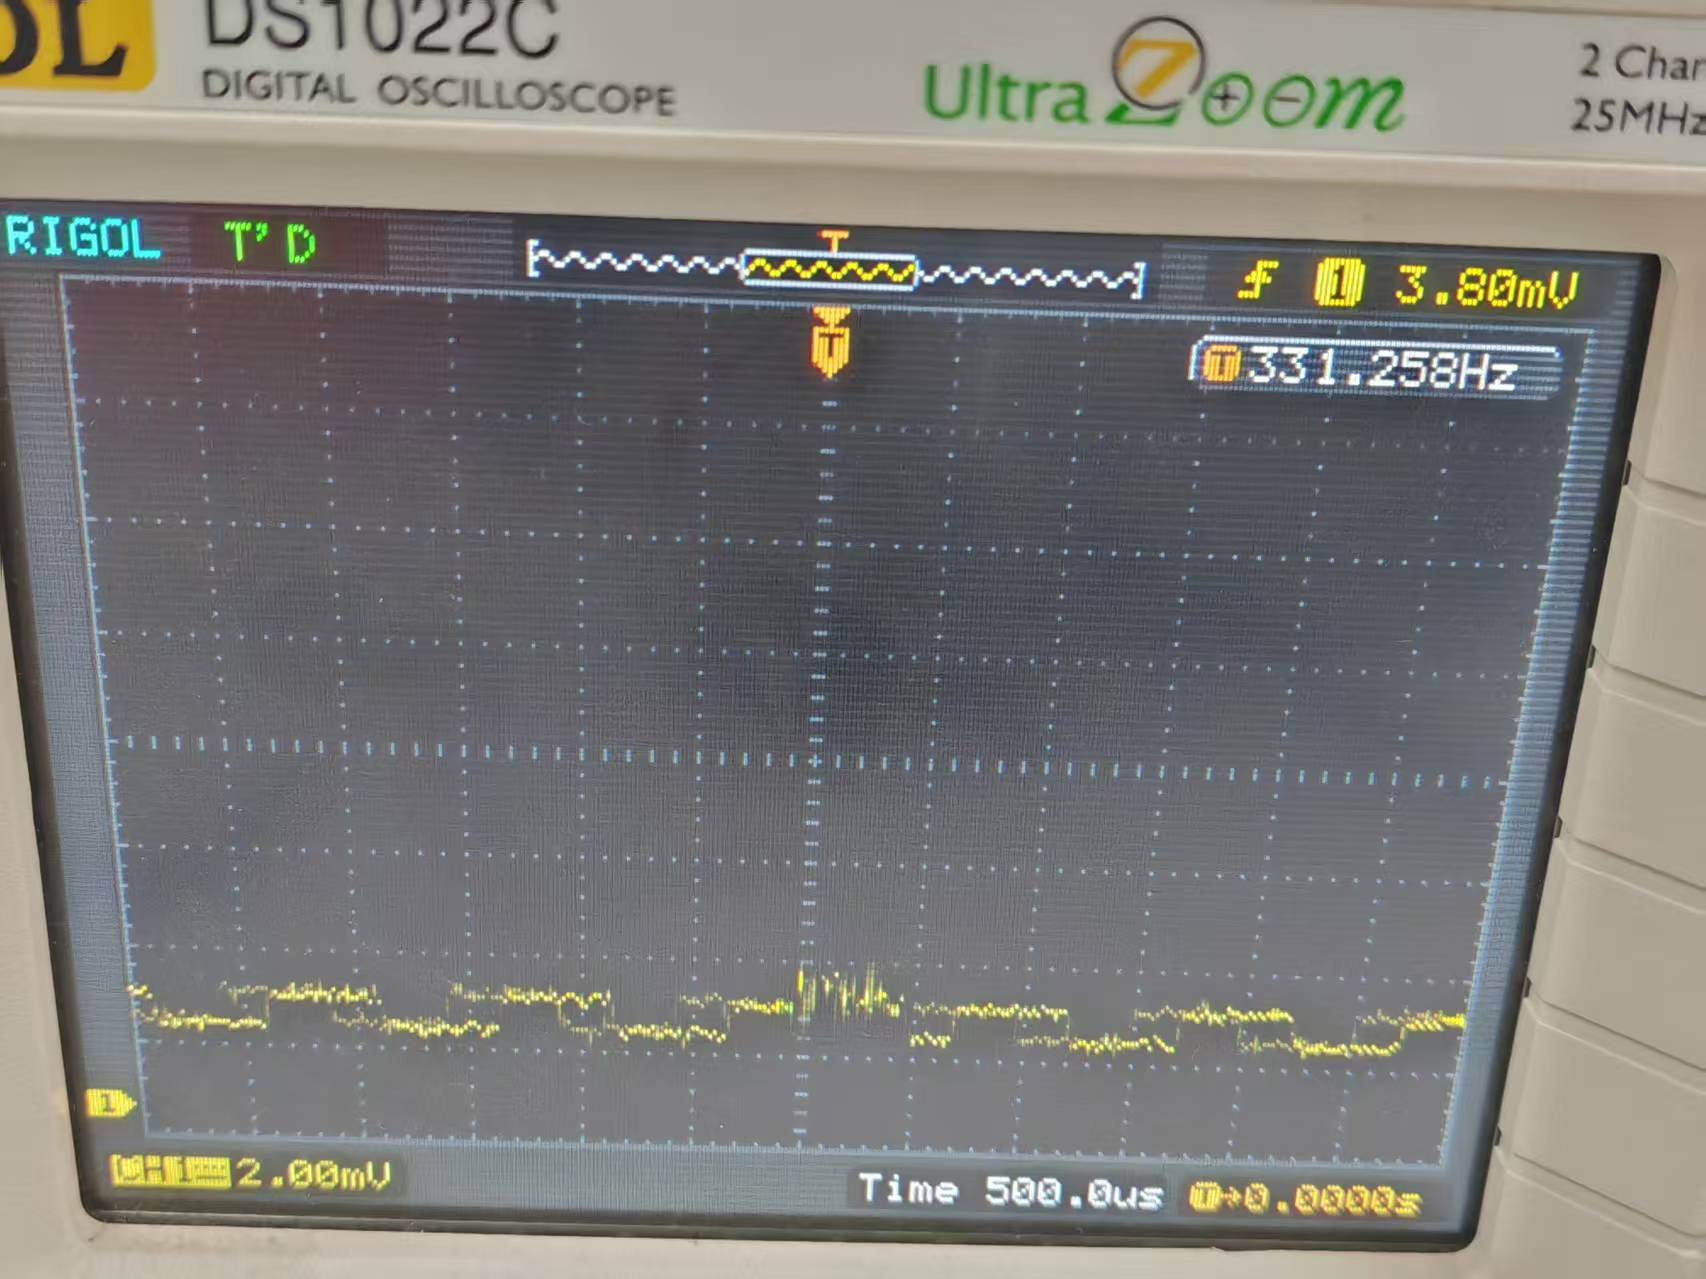
\includegraphics[width=.95\linewidth]{figures/p42.jpg}
        \caption{调节销钉}
        \label{fig:best-match}
    \end{minipage}%
    \begin{minipage}{.24\textwidth}
        \centering
        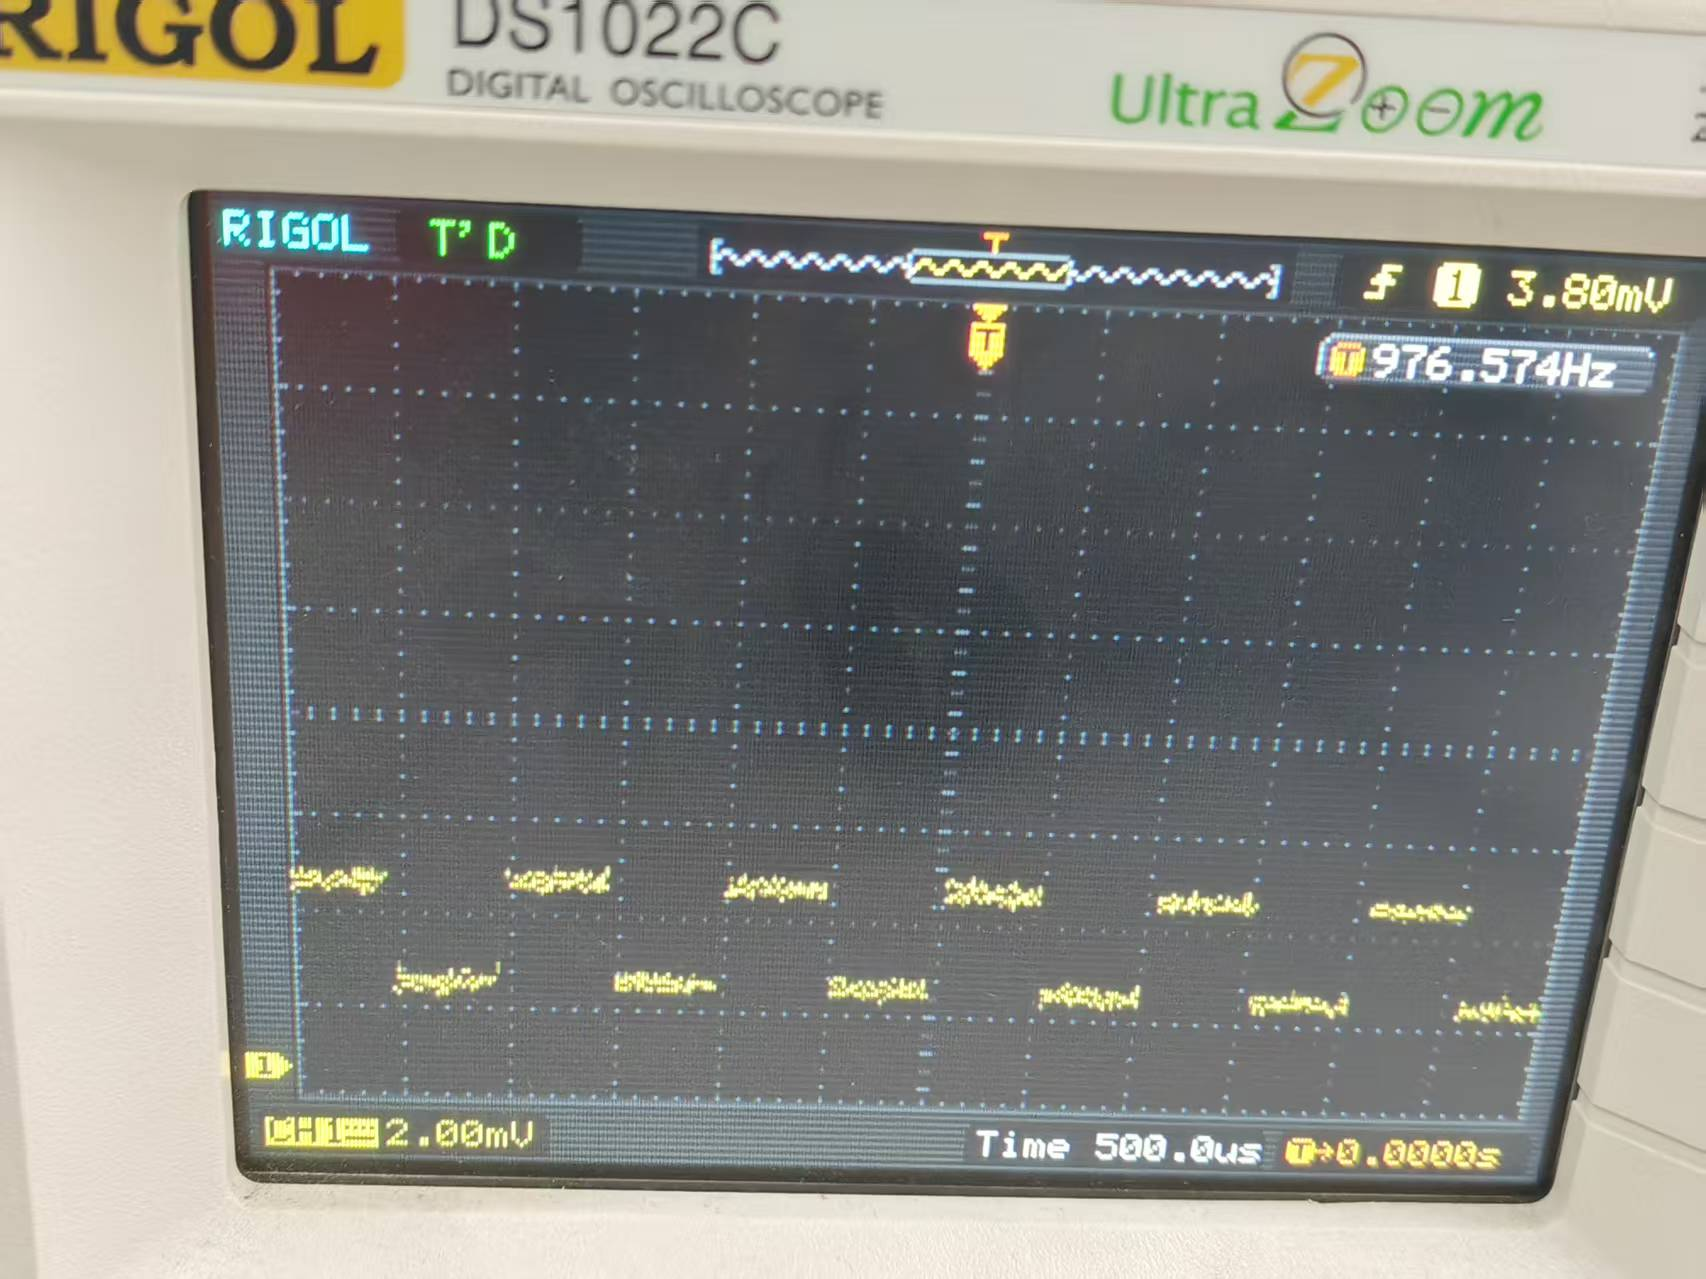
\includegraphics[width=.95\linewidth]{figures/p43.jpg}
        \caption{重复1}
        \label{fig:pmax-match1}
    \end{minipage}
    \begin{minipage}{.24\textwidth}
        \centering
        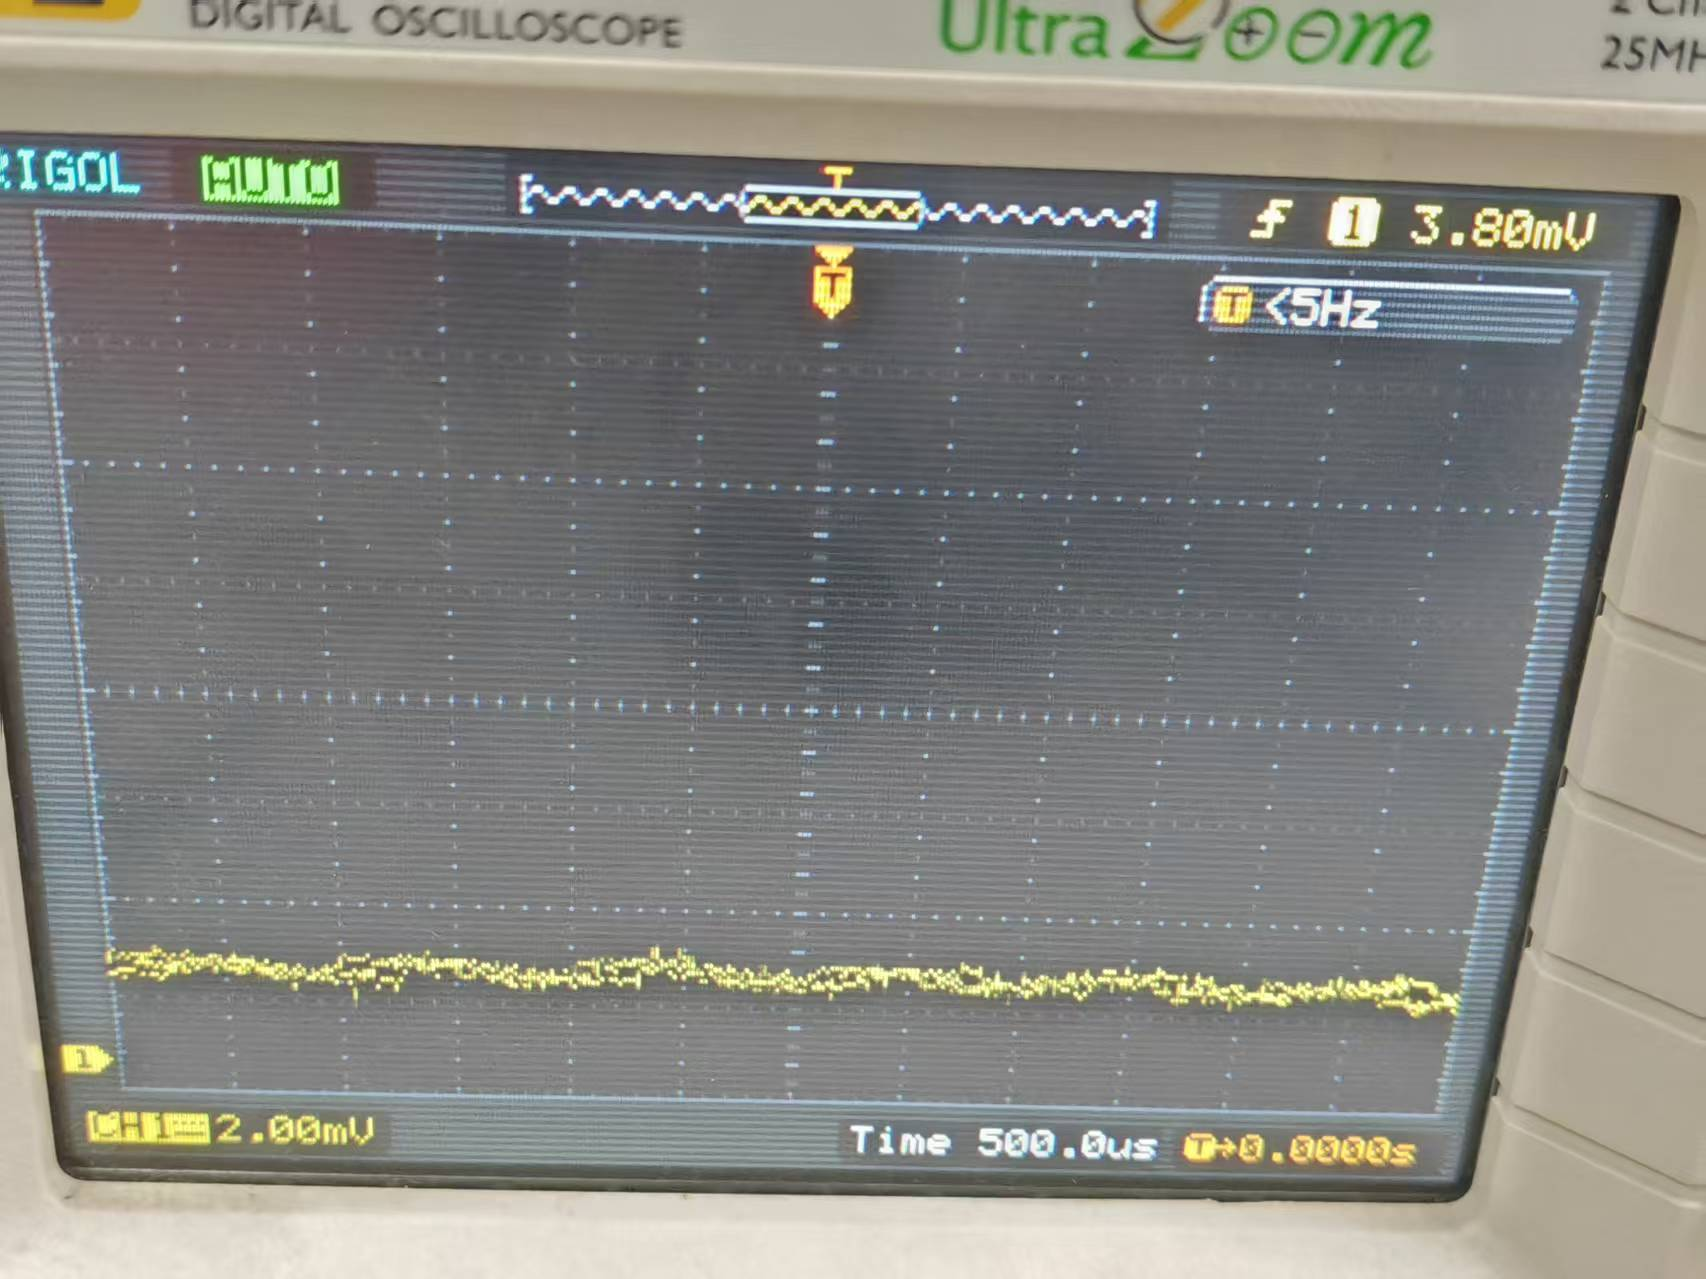
\includegraphics[width=.95\linewidth]{figures/p44.jpg}
        \caption{重复2}
        \label{fig:pmax-match1}
    \end{minipage}
\end{figure}


\begin{figure}[H]
    \centering
    \begin{minipage}{.24\textwidth}
        \centering
        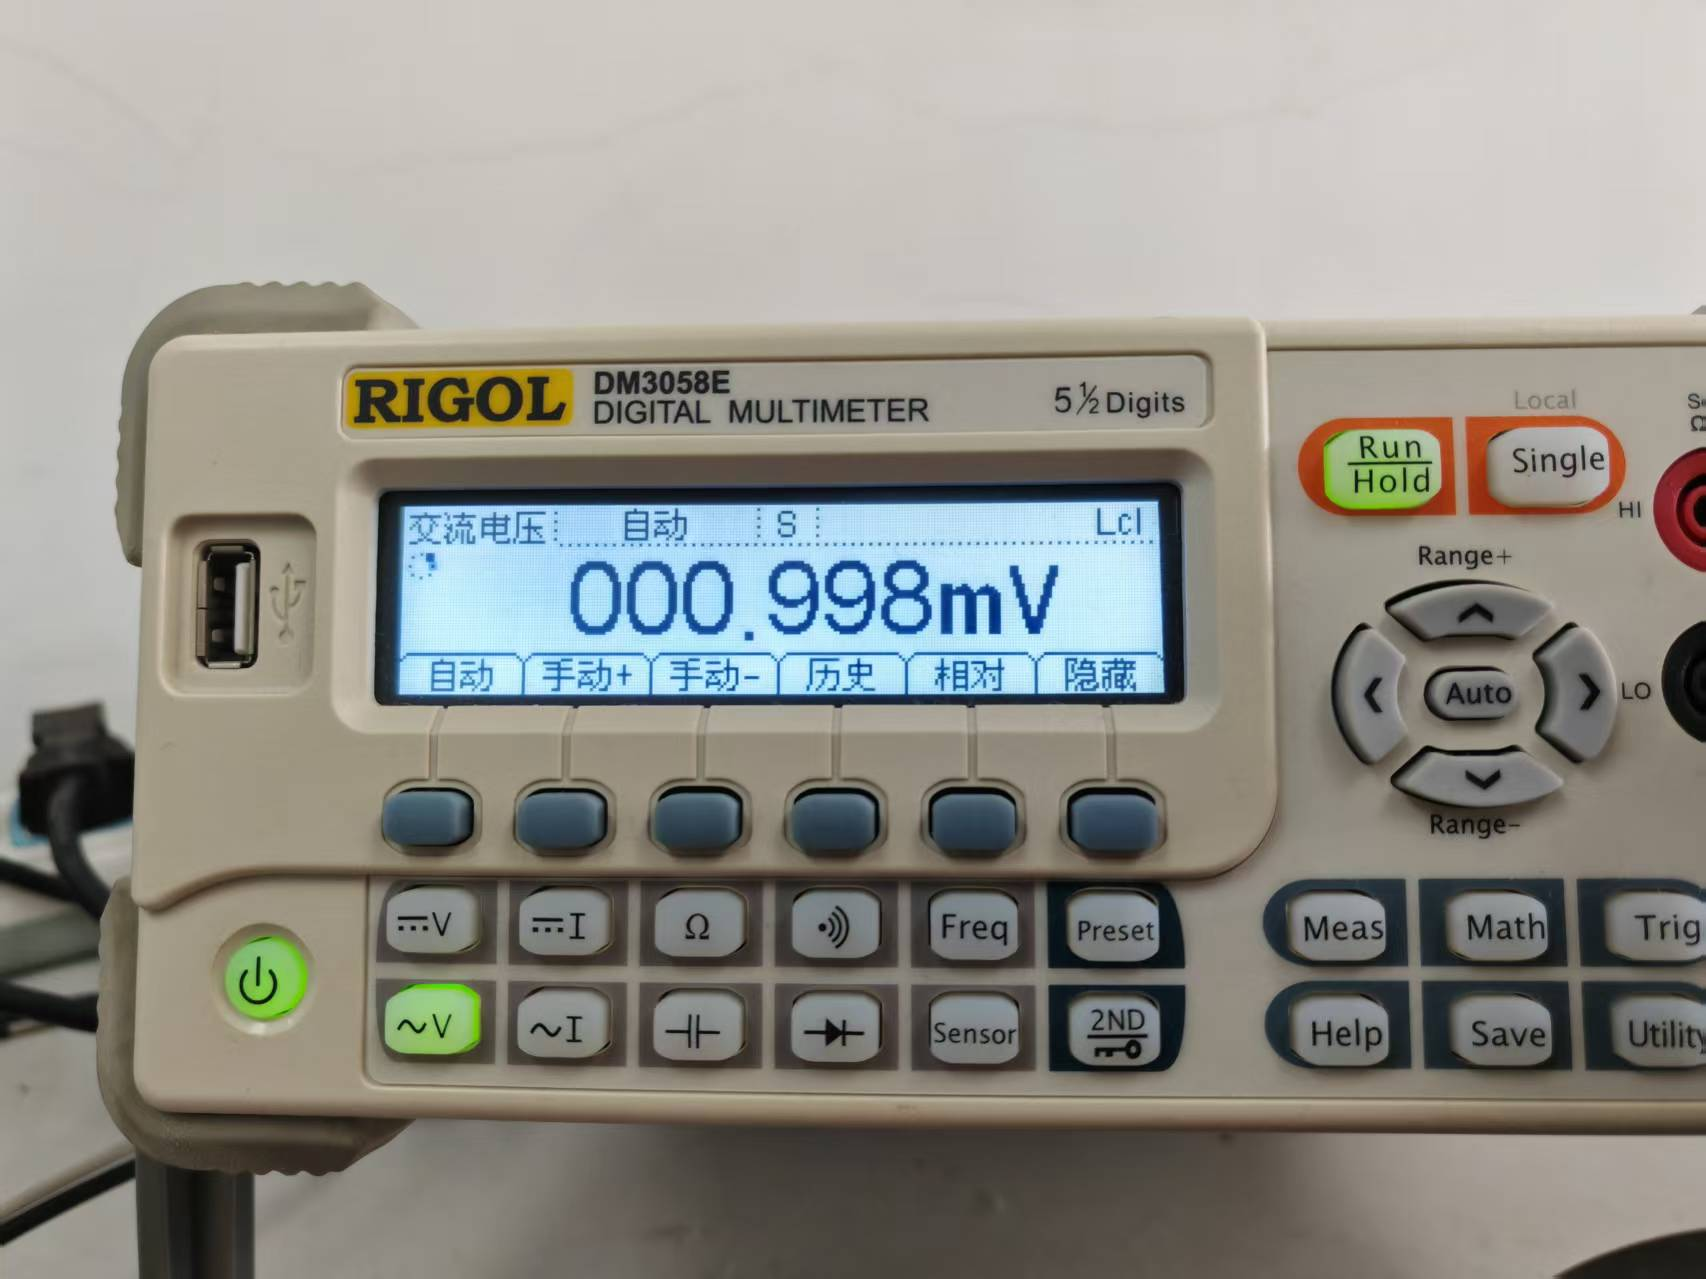
\includegraphics[width=.95\linewidth]{figures/p51.jpg}
        \caption{pmax1}
        \label{fig:pmin-match1}
    \end{minipage}%
    \begin{minipage}{.24\textwidth}
        \centering
        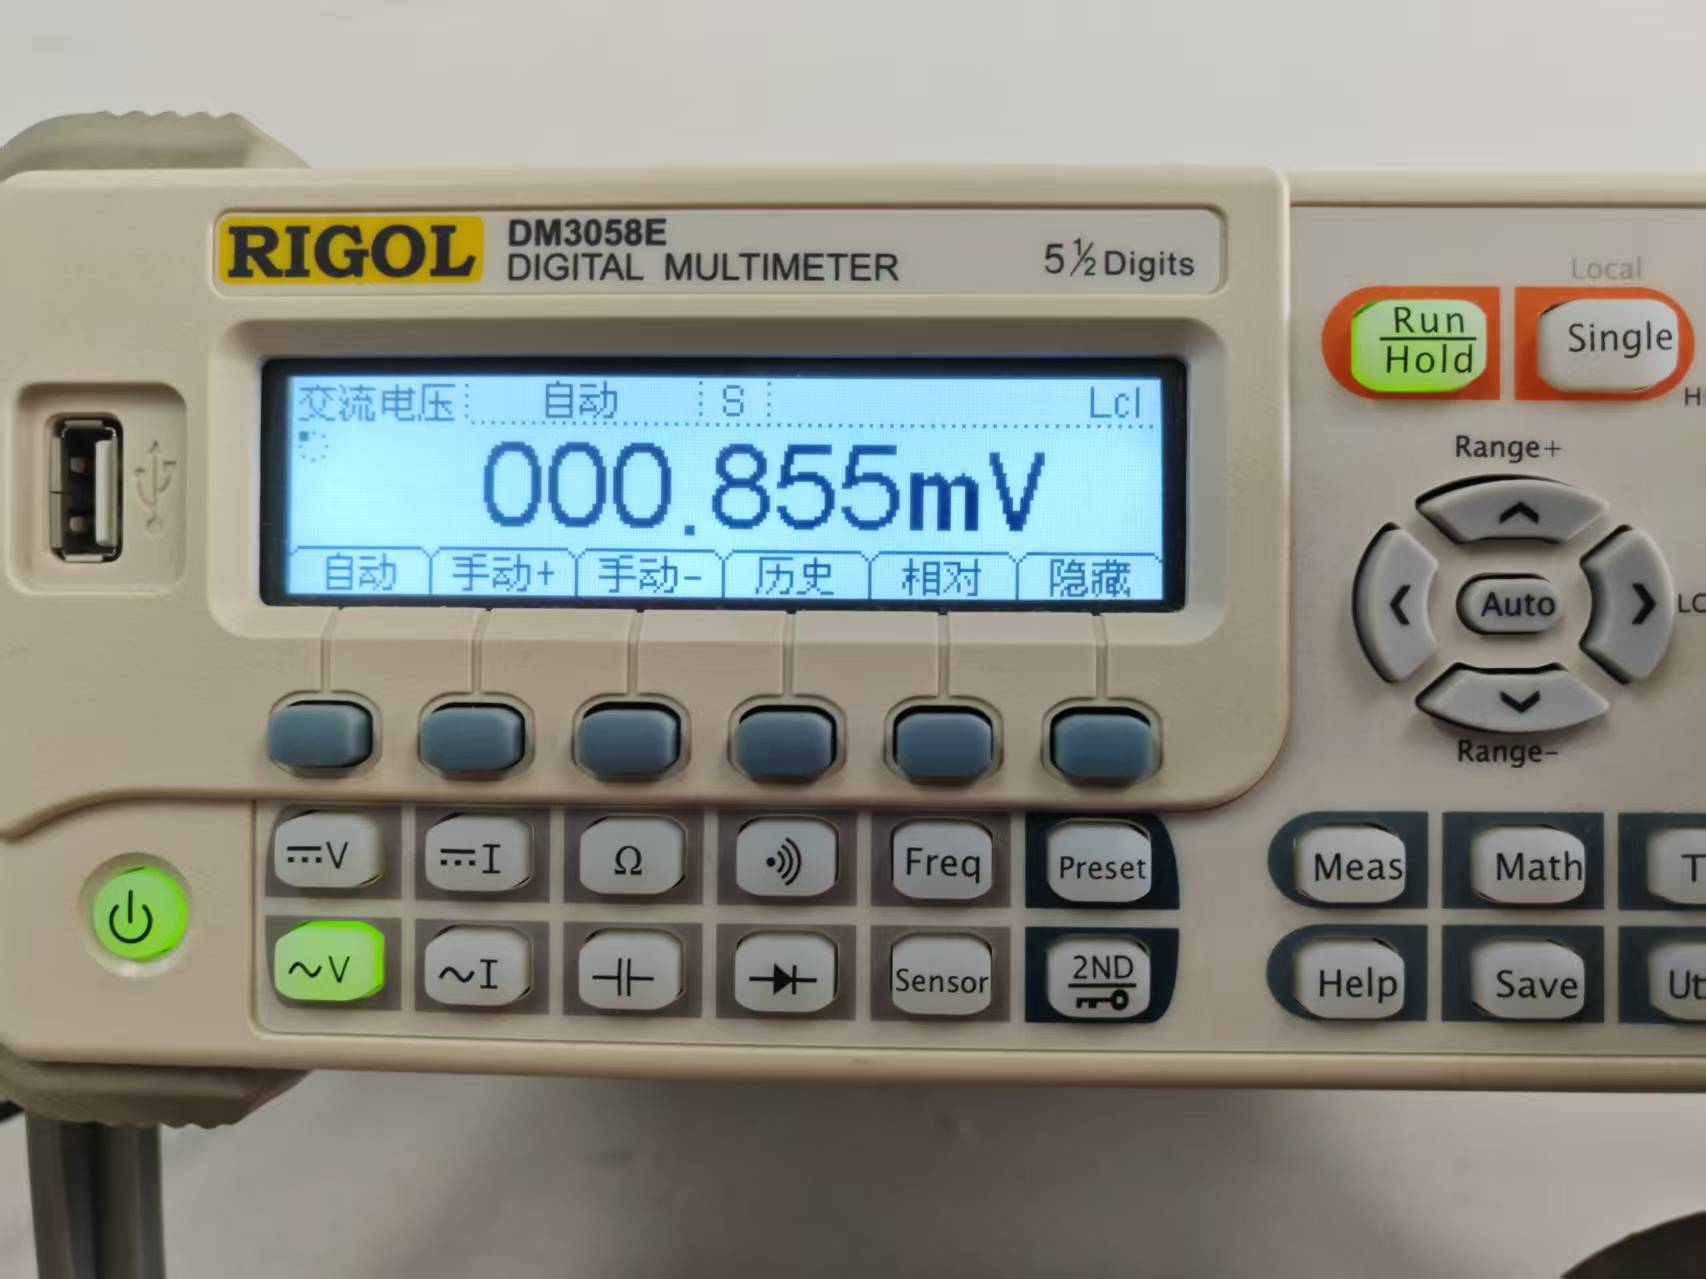
\includegraphics[width=.95\linewidth]{figures/p52.jpg}
        \caption{pmin1}
        \label{fig:pmax-match2}
    \end{minipage}%
    \begin{minipage}{.24\textwidth}
        \centering
        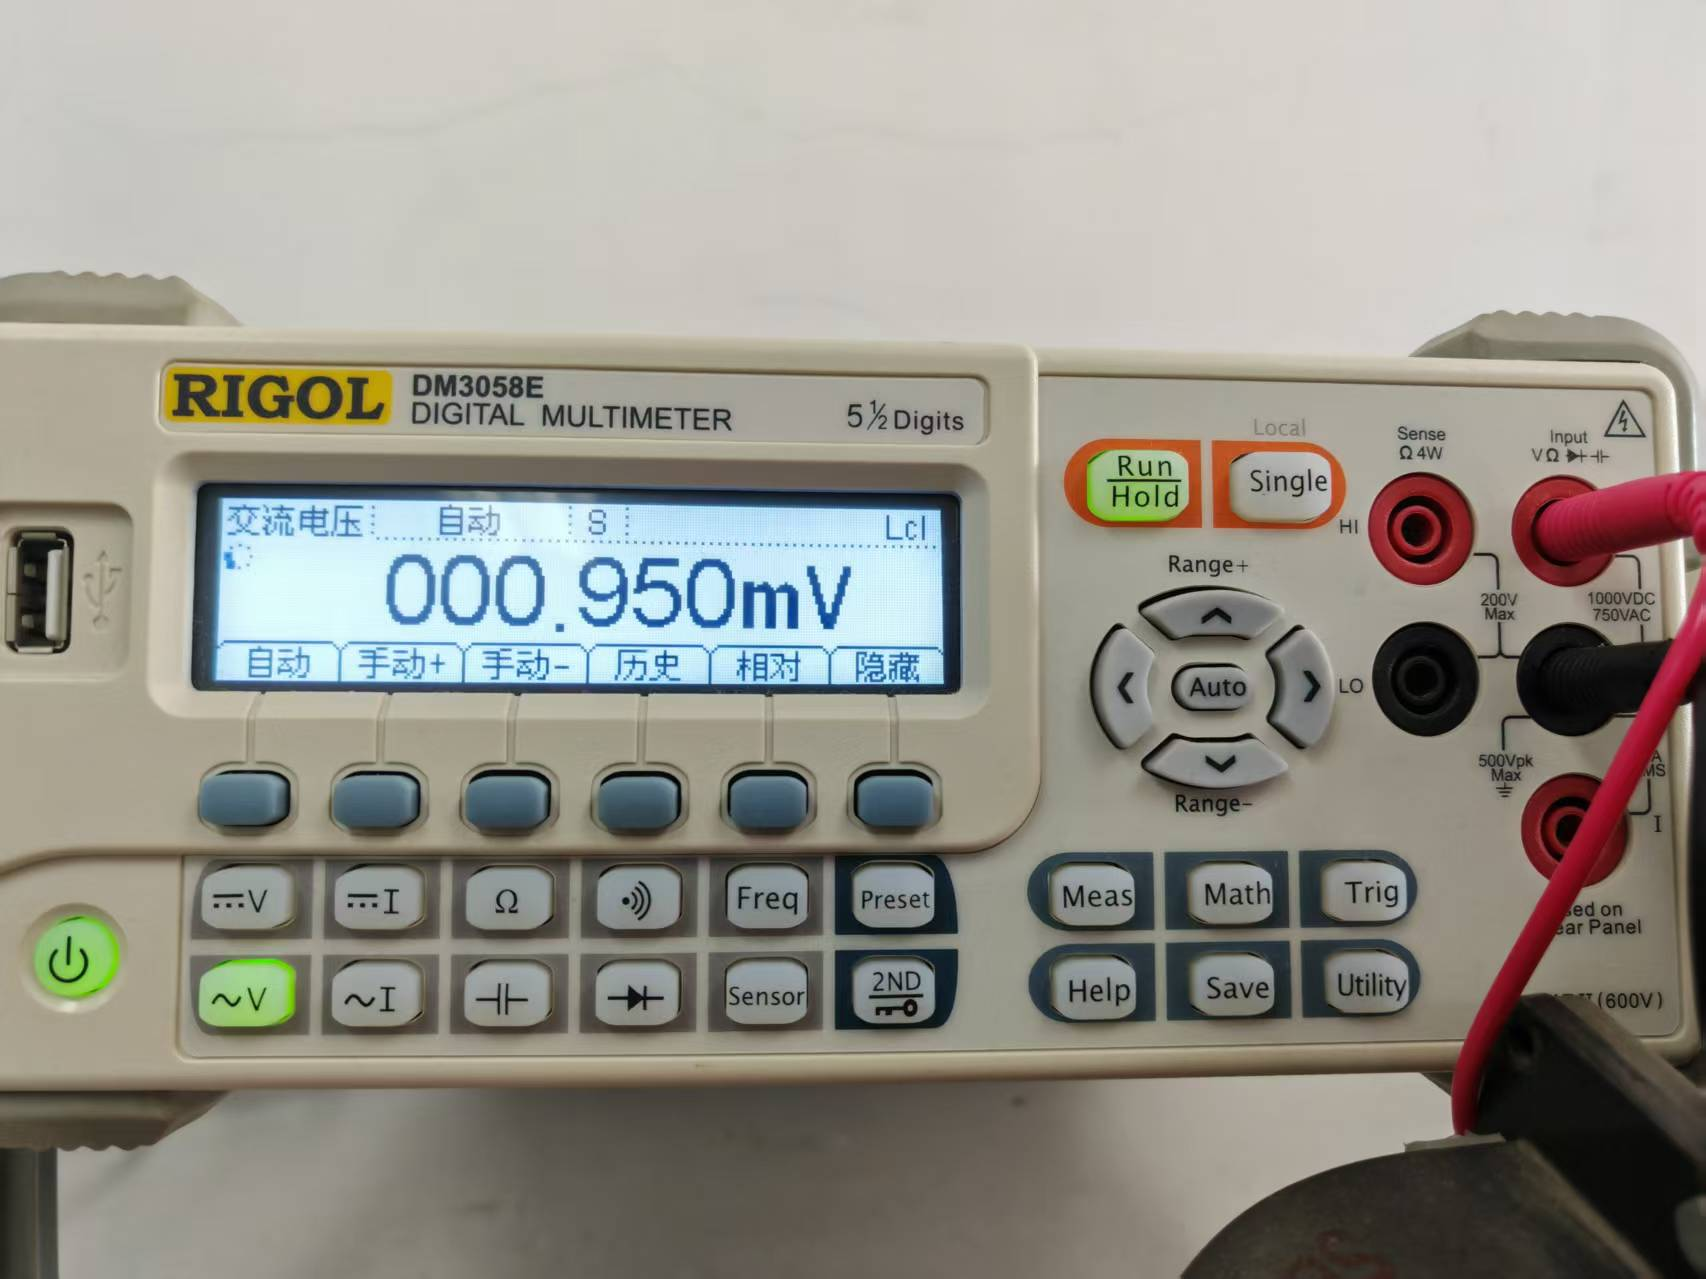
\includegraphics[width=.95\linewidth]{figures/p53.jpg}
        \caption{pmax2}
        \label{fig:pmin-match2}
    \end{minipage}
    \begin{minipage}{.24\textwidth}
        \centering
        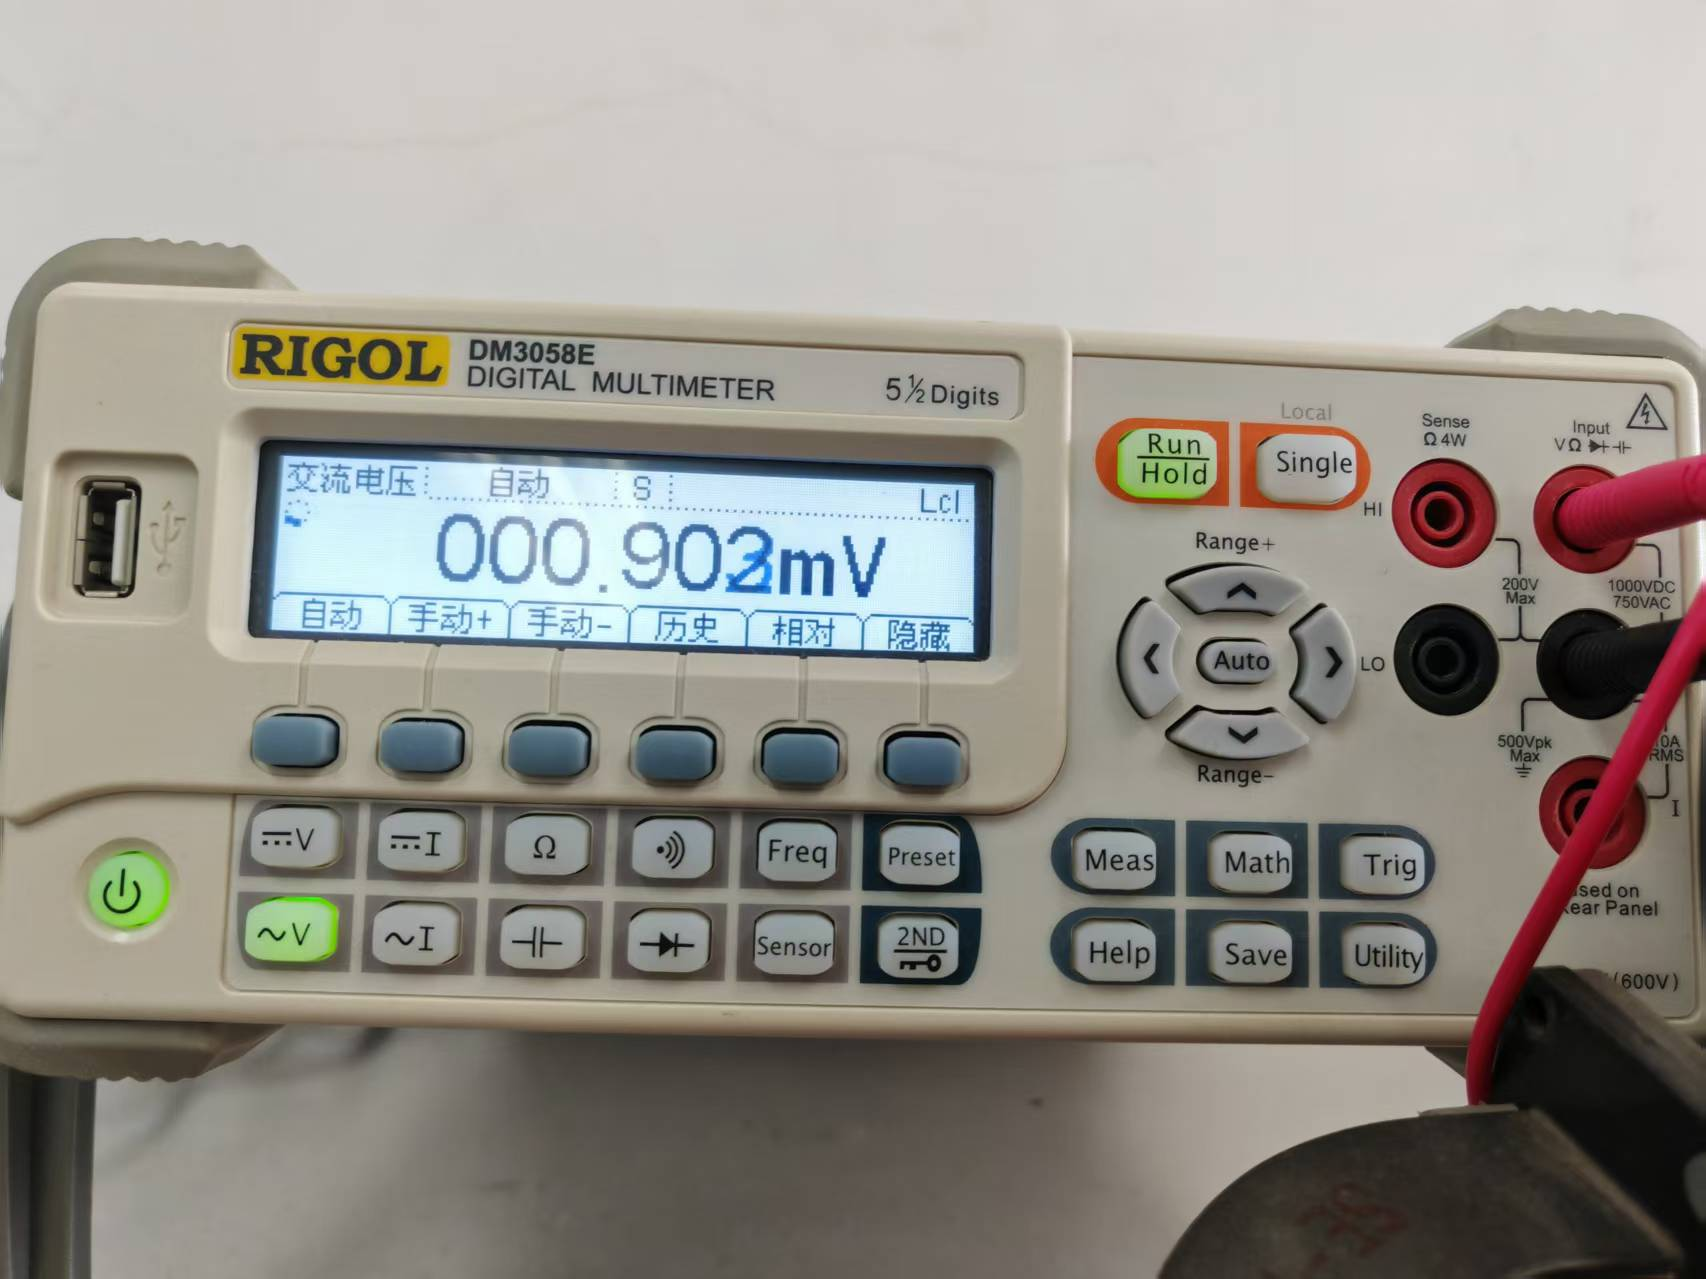
\includegraphics[width=.95\linewidth]{figures/p54.jpg}
        \caption{pmin2}
        \label{fig:pmin-match2}
    \end{minipage}
\end{figure}

测试值为：

$P_{max\text{(匹配 1)}}=0.998mV$,$P_{min\text{(匹配 1)}}=0.855mV$

$P_{max\text{(匹配 2)}}=0.950mV$,$P_{min\text{(匹配 2)}}=0.903mV$

\newpage

\section{实验报告内容要求}

\subsection{根据实测值计算波导波长$\lambda_g$}

    $\lambda_g=2(d_{min2}-d_{min1})=2(5.960-3.700)=4.520cm$
\subsection{计算实测频率下矩形波导 TE10 模的波导波长$\lambda_g$的理论值，并与实验测量值比较}
    
    $\lambda=\frac{c}{f} = \frac{3 \times 10^{10}}{9.396 \times 10^{9}} = 3.193cm$
    $\lambda_g= \frac{\lambda}{\sqrt{1-(\frac{\lambda}{2a})^{2}}} = \frac{3.193}{\sqrt{1-(\frac{3.193}{2 \times 2.286})^{2}}} = 4.461cm$
   
    实测值与理论值相差0.059cm，相对误差为1.32\%
    \subsection{计算容性膜片+匹配负载时的驻波系数$\rho$,在 Smith 圆图上读出容性膜片+匹配负载的反射系数$\Gamma$ 和归一化阻抗值}
    

    $\rho=\sqrt[]{\frac{P_{max}}{P_{min}}}=\sqrt{\frac{0.215}{0.045}}=2.186$

    $|\Gamma(0)| = \frac{\rho - 1}{\rho + 1} = \frac{2.186 - 1}{2.186 + 1} = 0.372$

    
    由$\Delta d = d_{min1\text{(短)}}-d_{min1\text{(膜片)}}=0.495cm = \frac{\psi(0)\lambda_g}{4 \pi} + \frac{\lambda_g}{4} \quad (\lambda_g \text{用} \text{cm} \text{作单位})$

    可得$\psi(0)=-1.765=-101.1 ^{\circ} $ 
    
    如图，由smith圆图，$Z=0.672-0.569j$

    \begin{figure}[H]
    \centering
    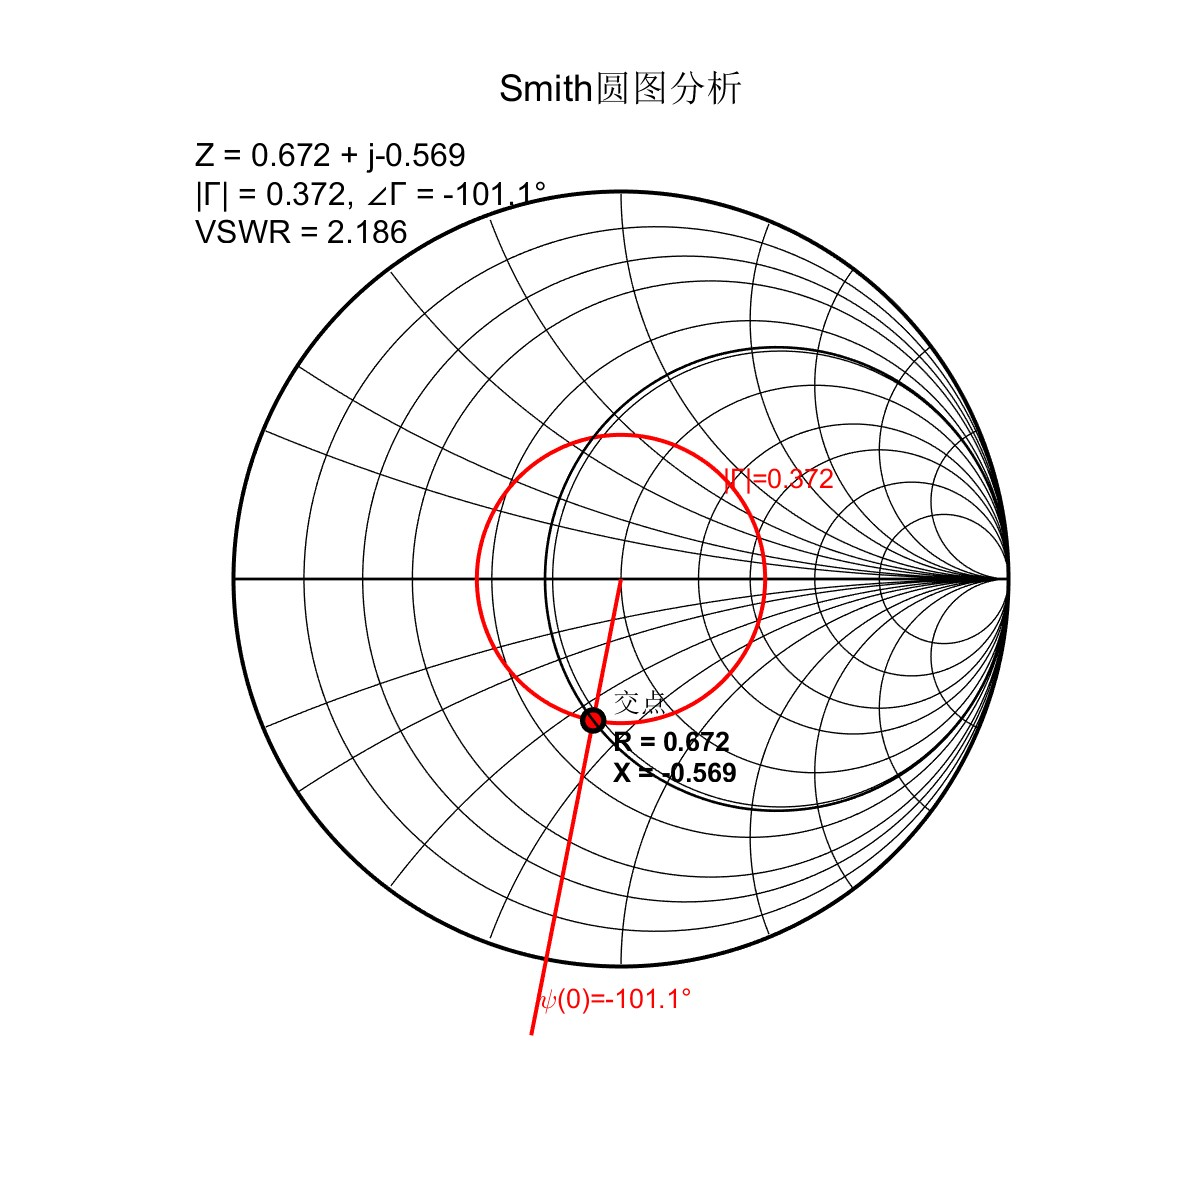
\includegraphics[width=0.5\linewidth]{figures/smith1.jpg} % 数字表示放缩比例
    \caption{Smith 圆图分析}
    \end{figure}

    \subsection{计算用单销钉调节匹配后的驻波系数$\rho$并与负载为匹配负载时的驻波系数$\rho$匹配比较}
    
    $\rho=\sqrt[]{\frac{P_{max\text{(匹配 1)}}}{P_{min\text{(匹配 1)}}}}=\sqrt{\frac{0.998}{0.855}}=1.080$

    $\rho\text{(匹配负载)}=\sqrt[]{\frac{P_{max\text{(匹配 2)}}}{P_{min\text{(匹配 2)}}}}=\sqrt{\frac{0.950}{0.903}}=1.026$

    
    【匹配比较】：驻波系数越接近1则匹配效果越好，故说明单销钉调节匹配后的效果弱于匹配负载时的匹配效果，可能是由于单销钉调节匹配时销钉位置不够精确，或者是由于单销钉调节器的损耗引起的。
\subsection{量出单销钉调配器销钉到负载的长度，计算匹配状态时销钉所呈现的归一化电抗值。借用圆图说明此时系统为什么匹配}
首先计算传输线的电长度：
\begin{equation}
    \beta d = \frac{2\pi d}{\lambda_g} = \frac{2\pi \times 6.8481}{4.520} \approx 9.51942 \, \text{rad}
\end{equation}
对 $2\pi$ 取模后得到实际相位角：
\begin{equation}
    \beta d \pmod{2\pi} = 9.51942 - 1 \times 2\pi \approx 9.51942 - 6.28319 \approx 3.23623 \, \text{rad} \quad (\approx 185.43^\circ)
\end{equation}
计算其正切值：
\begin{equation}
    \tan(\beta d) = \tan(3.23623 \, \text{rad}) \approx 0.09492
\end{equation}

已知负载的归一化阻抗为 $z_L = 0.672 - 0.569j$。
则对应的归一化导纳为：
\begin{equation}
    y_L = \frac{1}{z_L} = \frac{1}{0.672 - 0.569j} \approx 0.86600 + 0.73400j
\end{equation}

通过传输线变换至销钉位置的导纳 $y_d = g_d + jb_d$ 为：
\begin{equation}
    y_d = \frac{y_L + j\tan(\beta d)}{1 + j y_L \tan(\beta d)} = \frac{(0.86600 + 0.73400j) + j(0.09492)}{1 + j(0.86600 + 0.73400j)(0.09492)}
\end{equation}
化简得（根据数值计算结果）：
\begin{equation}
    y_d \approx 1.00172 + 0.80247j
\end{equation}
即 $g_d \approx 1.00172$，$b_d \approx 0.80247$。

为了实现匹配（总导纳为 1），销钉需提供以下并联电纳。销钉提供的电纳 $jB_{stub}$ 用于抵消 $y_d$ 的虚部，使得最终导纳的实部尽可能接近1。
即 $y_d + jB_{stub} = g_d$。因此 $B_{stub} = -b_d$。
\begin{equation}
    B_{stub} = -b_d \approx -0.80247
\end{equation}
对应的归一化电抗值为：
\begin{equation}
    X_{stub} = \frac{1}{B_{stub}} \approx \frac{1}{-0.80247} \approx -1.24610
\end{equation}

\medskip
\noindent\textbf{匹配原理分析（Smith 圆图说明）：}\\
在 Smith 圆图上，匹配过程如下所示：

\begin{itemize}
    \item \textbf{点 A（负载导纳）}：$ y_L = 0.86600 + 0.73400j $，对应负载原始导纳。
    \item \textbf{点 B（传输线变换后导纳）}：从 $y_L$ 点沿等反射系数模值圆（向着发生器方向）旋转电长度 $d/\lambda_g = 6.8481/4.520 \approx 1.51507$ 个波长（对应角度约为 $1.51507 \times 360^\circ \approx 545.43^\circ$，即 $545.43^\circ - 360^\circ = 185.43^\circ$ 的旋转）至点 $y_d \approx 1.00172 + 0.80247j $。
    \item \textbf{点 C（加入销钉后导纳）}：在 $y_d$ 点并联纯电纳 $jB_{stub} \approx -0.80247j$。在Smith圆图上，这是沿着等电导圆 $G \approx 1.00172$ 移动，消除虚部，到达点 $y_{final} = g_d \approx 1.00172$。此点非常接近匹配点 $y=1$（圆图中心）。
\end{itemize}
 
\begin{figure}[H]
    \centering
    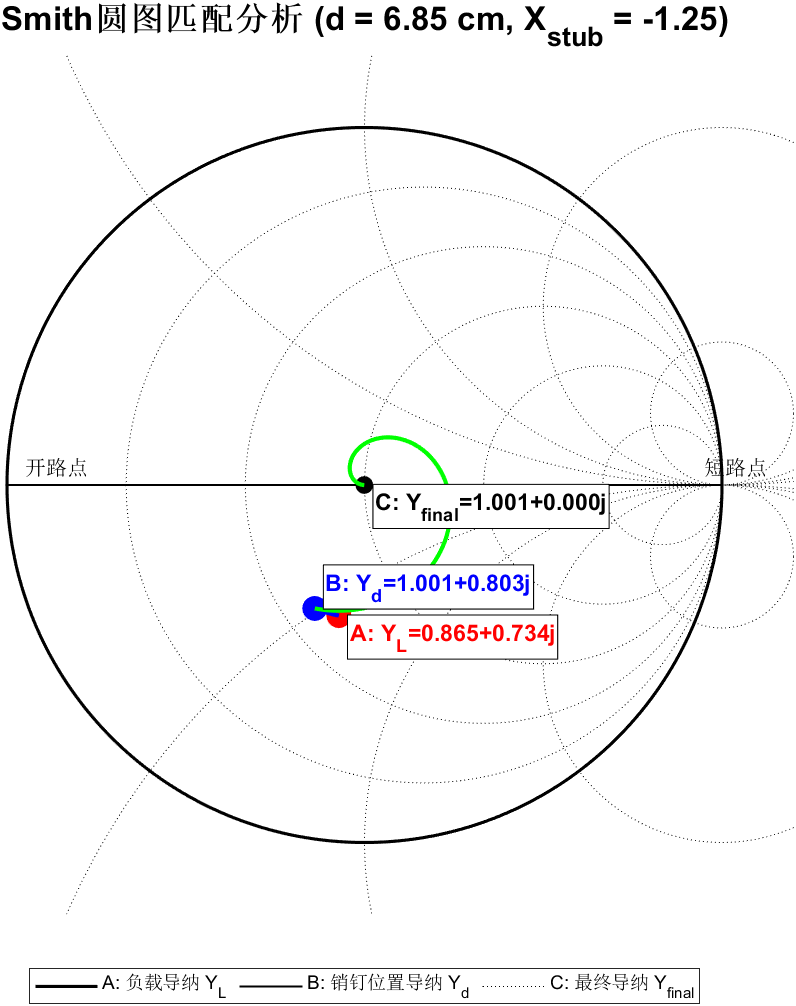
\includegraphics[width=0.5\linewidth]{figures/smith2.png} % 数字表示放缩比例
    \caption{Smith 圆图分析}
    \end{figure}

\textbf{匹配效果验证：}\\
根据实测驻波比 $\rho = 1.080$，可计算反射系数幅值：
\begin{equation}
    |\Gamma(0)| = \frac{\rho - 1}{\rho + 1} = \frac{1.080 - 1}{1.080 + 1} = 0.038
\end{equation}
该值较小，表明反射显著降低，验证了匹配效果。

综上所述，系统通过引入销钉电纳抵消导纳虚部，使得输入端口接近匹配状态，从而有效降低了反射系数。

\section{回答问题}
\subsection{测量线开口端不接短路块，任意接一负载，能否测出波导波长？接短路块测波导波长有什么优点？}
\textbf{能否测出}：可以测出波导波长。无论终端接何种负载（除非是理想匹配负载），传输线上一般都会形成驻波。通过测量相邻两个电压波腹点（或波节点）之间的距离，这个距离总是等于半个波导波长 ($\lambda_g/2$)。因此，可以推算出波导波长 $\lambda_g$。

\textbf{接短路块的优点}：
\begin{itemize}
    \item \textbf{驻波特性显著}：短路块会造成全反射，使得电压驻波比 ($\rho$) 趋近于无穷大。这使得电压的波峰和波谷（即波腹点和波节点）非常分明，便于更精确地确定波节点的位置。
    \item \textbf{波节点位置清晰}：短路面本身就是一个确定的电压波节点，从该点开始可以清晰地找到一系列等间距的波节点，从而提高了测量精度。
\end{itemize}

\subsection{测负载驻波相位为什么要先测$d_{min1\text{(短)}}?$}
测量负载驻波相位时，先测量 $d_{min1(\text{短})}$（即测量线开口端接短路块时，第一个电压波节点的位置）是为了确定一个\textbf{参考基准面}，也称为等效短路面位置。

当接入待测负载后，会形成新的驻波分布，从而测得新的第一个电压波节点位置 $d_{min1(\text{负载})}$。这个新的波节点位置相对于之前测得的基准面位置会有一个偏移。这个偏移量 $\Delta d = |d_{min1(\text{负载})} - d_{min1(\text{短})}|$ 与波导波长 $\lambda_g$ 结合，可以用来计算负载的反射系数相位角 $\psi(0)$，进而通过Smith圆图或计算得到负载的归一化阻抗值。具体来说，反射系数相位角 $\psi(0)$ 与波节点位置的关系由公式 $d_{min1} = \frac{\psi(0)\lambda_g}{4\pi} + \frac{\lambda_g}{4}$ (\text{cm}) (当 $\psi(0)$ 的范围导致 $d_{min1}$ 为正值时，$\lambda_g$ 用cm作单位) 给出。通过比较有负载和短路时的 $d_{min1}$ 即可求解相位信息。

\subsection{单销钉调配器调节匹配时，为什么检波器输出指示越小，表示调配得越好？}
在实验装置中，定向耦合器通常被反向接入，用于对主波导中的\textbf{反射功率}进行采样。波导检波器连接在定向耦合器的耦合臂（副波导）输出端，其输出信号大小反映了主波导中反射波功率的大小。

当单销钉调配器调节得当时，系统趋向于阻抗匹配。理想匹配状态下，负载反射的功率最小（理论上为零）。因此，定向耦合器采样到的反射功率也最小，从而导致波导检波器的输出指示（例如，示波器上显示的检波信号幅度或数字万用表上的读数）最小。所以，检波器输出指示越小，表明反射回来的功率越小，系统的匹配状态就越好。

\subsection{如果经销钉调配器调配后，测得驻波系数$\rho=1$,在单销钉调配器与负载之间是否是行波？单销钉调配器至信号源方向是否是行波？为什么？}
\begin{itemize}
    \item \textbf{在单销钉调配器与负载之间}：\textbf{一般不是行波}（除非负载本身恰好是匹配的，即 $Z_L = Z_0$，这种情况下无需调配器）。单销钉调配器的作用是在其接入点引入一个特定的并联电纳（或电抗）。这个引入的电纳与从调配器位置看进去的、由“传输线+负载”构成的等效导纳（或阻抗）相结合，使得调配器输入端的总导纳（或阻抗）等于传输线的特性导纳（或阻抗）。这意味着，为了抵消原来的失配，调配器本身及其到负载的这一段传输线上仍然存在由负载引起的反射波，这些反射波与入射波叠加形成驻波。只有当负载本身就是匹配的时候，这段区间才是行波。

    \item \textbf{单销钉调配器至信号源方向}：\textbf{是行波}。当通过单销钉调配器成功实现匹配，使得测得的驻波系数 $\rho=1$ 时，这意味着从调配器位置向信号源方向看过去的输入阻抗 $Z_{in}$ 等于传输线的特性阻抗 $Z_0$。根据传输线理论，当一段传输线的输入端呈现为其特性阻抗时，表明该段传输线上没有发生反射（或者说入射波被完全“吸收”）。因此，从信号源到单销钉调配器这一段传输线上，电磁波以行波状态传播，没有反射波存在。
\end{itemize}
\section{实验总结与心得体会}
\subsection{实验总结}

本次波导传输线特性测量与阻抗匹配实验中，我进行了细致的操作和数据分析，主要总结如下：

\subsubsection{工作频率与波导波长测量}
成功测定了系统的工作频率 $ f $ 为 \textbf{9.396 GHz}。

通过测量驻波线上相邻两个波节点的位置（$d_{\min1} = 3.700\,\text{cm}$，$d_{\min2} = 5.960\,\text{cm}$），计算得到实验波导波长：
$$
\lambda_g = 2 \times (d_{\min2} - d_{\min1}) = 4.520\,\text{cm}
$$

基于实测频率，计算得到 TE10 模的理论波导波长为 $4.461\,\text{cm}$，与实测值的相对误差为 \textbf{1.32\%}，符合理论预期。

\subsubsection{容性膜片负载特性分析}
测量了容性膜片+匹配负载的特性，确定了短路参考面位置：$d_{\min1(\text{短})} = 6.180\,\text{cm}$ 和负载条件下的波节点位置：$d_{\min1(\text{膜片})} = 5.685\,\text{cm}$。

测得的最小和最大相对功率分别为：$P_{\min} = 0.045\,\text{mV}$ 和 $P_{\max} = 0.215\,\text{mV}$，由此计算出驻波系数：
$$
\rho = \frac{P_{\max}}{P_{\min}} = 2.186
$$

根据驻波系数和波节点位移，计算得到反射系数模值：
$$
|\Gamma(0)| = \frac{\rho - 1}{\rho + 1} = \frac{2.186 - 1}{2.186 + 1} \approx 0.372
$$
相位角为：
$$
\psi(0) = -101.1^\circ
$$

在 Smith 圆图上确定了归一化负载阻抗约为：
$$
Z = 0.672 - 0.569j
$$

\subsubsection{单销钉阻抗匹配}
通过调节单销钉的位置和插入深度，对容性膜片负载进行了匹配。匹配后测得：
$$
P_{\max(\text{匹配1})} = 0.998\,\text{mV}, \quad P_{\min(\text{匹配1})} = 0.855\,\text{mV}
$$
计算得到驻波系数：
$$
\rho = \frac{P_{\max}}{P_{\min}} = 1.080
$$

作为对比，直接接入匹配负载时测得的驻波系数为：
$$
\rho = 1.026
$$
说明单销钉匹配效果略逊于理想匹配负载，可能与调节精度和调配器自身损耗有关。

根据选定的销钉到负载距离 $d = 6.8481\,\text{cm}$（此为报告中用于理论计算演示的值，非本次实验直接测量值，但用于说明原理），计算了销钉在该“匹配状态”下所呈现的归一化电抗值：
$$
X_{\text{stub}} \approx -1.246
$$

并通过 Smith 圆图演示了从 $y_L$ 变换到 $y_d$，再通过销钉补偿到接近匹配点 $y = 1$ 的过程。
\subsection{实验心得体会}
这次实验让我对波导传输线的工作原理、史密斯圆图的应用以及阻抗匹配技术有了更为直观和深刻的理解。课本上的公式和理论，在亲手操作和调试中变得鲜活起来。
通过本次实验，我不仅巩固了理论知识，更锻炼了动手操作和分析解决问题的能力。特别是对阻抗匹配“化腐朽为神奇”的过程有了更深的体会——一个原本反射很大的系统，通过小小的销钉就能调整到接近全吸收的状态，这正是电磁理论与工程应用的魅力所在。希望未来能有更多这样的机会，将理论应用于实践，不断提升自己的专业素养。

\section{绘图所用Matlab代码}
\begin{lstlisting}[language=matlab, caption=Smith1 Code]
function smithchart2()
    Z1 = 0.672 - 0.569j;  
    
    absGamma2 = 0.038;
    psi2 = 0;
    Gamma2 = absGamma2 * exp(1i * psi2);
    
    Z2 = (1 + Gamma2) / (1 - Gamma2);
    
    figure('Position', [100, 100, 600, 600], 'Color', 'white');
    hold on;
    axis equal;
    axis([-1.2 1.2 -1.2 1.2]);
    axis off;
    
    drawBasicSmithChart();
    
    Gamma1 = (Z1 - 1) / (Z1 + 1);
    
    plot(real(Gamma1), imag(Gamma1), 'ro', 'MarkerSize', 10, 'LineWidth', 2);
    text(real(Gamma1) + 0.05, imag(Gamma1) + 0.05, '容性膜片+匹配负载', 'FontSize', 10, 'Color', 'r');
    
    plot(real(Gamma2), imag(Gamma2), 'go', 'MarkerSize', 10, 'LineWidth', 2);
    text(real(Gamma2) + 0.05, imag(Gamma2) + 0.05, '容性膜片+单销钉(匹配)', 'FontSize', 10, 'Color', 'g');
    
    arrow_x = [real(Gamma1), real(Gamma2)];
    arrow_y = [imag(Gamma1), imag(Gamma2)];
    quiver(arrow_x(1), arrow_y(1), arrow_x(2)-arrow_x(1), arrow_y(2)-arrow_y(1), 0, 'MaxHeadSize', 0.5, 'LineWidth', 2, 'Color', 'b');
    
    Y1 = 1/Z1;
    
    beta_d = 78.75 * pi/180;
    
    Y2 = (Y1 + 1j*tan(beta_d))/(1 + 1j*Y1*tan(beta_d));
    
    Y_stub = -1j*imag(Y2);
    
    Y_total = real(Y2) + 1j*0;
    
    Z2_new = 1/Y_total;
    
    text(real(Gamma1) - 0.2, imag(Gamma1) - 0.1, ['Z = ' num2str(real(Z1), '%.3f') ' - j' num2str(abs(imag(Z1)), '%.3f')], 'FontSize', 10, 'FontWeight', 'bold');
    text(real(Gamma2) - 0.2, imag(Gamma2) - 0.1, ['Z \approx ' num2str(real(Z2_new), '%.3f')], 'FontSize', 10, 'FontWeight', 'bold');
    
    text(-1.1, 1.1, '阻抗匹配过程示意图', 'FontSize', 12);
    text(-1.1, 1.0, ['销钉提供导纳: Y_{stub} = j' num2str(imag(Y_stub), '%.3f')], 'FontSize', 12);
    text(-1.1, 0.9, ['销钉电抗: X_{stub} = ' num2str(-1/imag(Y_stub), '%.3f') 'j'], 'FontSize', 12);
    text(-1.1, 0.8, ['销钉距离负载: ' num2str(beta_d*180/pi, '%.1f') '°'], 'FontSize', 12);
    
    title('Smith圆图阻抗匹配分析', 'FontSize', 14);

    hold off;
end

function drawBasicSmithChart()
    theta = linspace(0, 2*pi, 1000);
    plot(cos(theta), sin(theta), 'k-', 'LineWidth', 1.5);
    
    plot([-1, 1], [0, 0], 'k-', 'LineWidth', 1);
    
    rValues = [0, 0.1, 0.2, 0.3, 0.5, 0.7, 1, 1.5, 2, 3, 5];
    for r = rValues
        center = [r/(1+r), 0];
        radius = 1/(1+r);
        
        theta = linspace(0, 2*pi, 200);
        x = center(1) + radius * cos(theta);
        y = center(2) + radius * sin(theta);
        
        plot(x, y, 'k-', 'LineWidth', 0.5);
    end
    
    xValues = [-5, -3, -2, -1.5, -1, -0.7, -0.5, -0.3, -0.2, 0.2, 0.3, 0.5, 0.7, 1, 1.5, 2, 3, 5];
    for x = xValues
        center_x = 1;
        center_y = 1/x;
        radius = abs(1/x);
        
        t = linspace(0, 2*pi, 500);
        circ_x = center_x + radius * cos(t);
        circ_y = center_y + radius * sin(t);
        
        mask = (circ_x.^2 + circ_y.^2) <= 1;
        
        if sum(mask) >= 2
            plot(circ_x(mask), circ_y(mask), 'k-', 'LineWidth', 0.5);
        end
    end
    
    plot(0, 0, 'ko', 'MarkerSize', 6, 'MarkerFaceColor', 'k');
    text(0.05, 0.05, '匹配点', 'FontSize', 10);
end

    \end{lstlisting}
\begin{lstlisting}[language=matlab, caption=Smith2 Code]
    function plot_matching_process_updated()
Z_L_val = 0.672 - 0.570j;
d_val = 6.8481;
lambda_g_val = 4.520;

beta_d_val = 2 * pi * d_val / lambda_g_val;
Y_L_val = 1 / Z_L_val;

t_beta_d = tan(beta_d_val);
Y_d_val = (Y_L_val + 1j*t_beta_d) / (1 + 1j*Y_L_val*t_beta_d);

B_stub_val = -imag(Y_d_val);

if B_stub_val == 0
    X_stub_val = Inf;
else
    X_stub_val = 1/B_stub_val;
end

Y_final_val = Y_d_val + 1j*B_stub_val;

figure('Position', [100, 100, 800, 800], 'Color', 'white');
hold on;
axis equal;
axis([-1.2 1.2 -1.2 1.2]);
axis off;

draw_basic_smith_chart();

Gamma_Y_L_val = (1 - Y_L_val) / (1 + Y_L_val);
Gamma_Y_d_val = (1 - Y_d_val) / (1 + Y_d_val);
Gamma_Y_final_val = (1 - Y_final_val) / (1 + Y_final_val);

plot(real(Gamma_Y_L_val), imag(Gamma_Y_L_val), 'ro', 'MarkerSize', 10, 'LineWidth', 2, 'MarkerFaceColor', 'r');
plot(real(Gamma_Y_d_val), imag(Gamma_Y_d_val), 'bo', 'MarkerSize', 10, 'LineWidth', 2, 'MarkerFaceColor', 'b');
plot(real(Gamma_Y_final_val), imag(Gamma_Y_final_val), 'ko', 'MarkerSize', 8, 'MarkerFaceColor', 'k');

draw_arc(Gamma_Y_L_val, Gamma_Y_d_val, 'b');
draw_arc(Gamma_Y_d_val, Gamma_Y_final_val, 'g');

text(real(Gamma_Y_L_val) + 0.03, imag(Gamma_Y_L_val) -0.06 , sprintf('A: Y_L=%.3f%+.3fj', real(Y_L_val), imag(Y_L_val)), 'FontSize', 11, 'FontWeight', 'bold', 'Color', 'r', 'BackgroundColor', 'w', 'EdgeColor','k', 'Margin', 1);
text(real(Gamma_Y_d_val) + 0.03, imag(Gamma_Y_d_val) + 0.06, sprintf('B: Y_d=%.3f%+.3fj', real(Y_d_val), imag(Y_d_val)), 'FontSize', 11, 'FontWeight', 'bold', 'Color', 'b', 'BackgroundColor', 'w', 'EdgeColor','k', 'Margin', 1);
text(real(Gamma_Y_final_val) + 0.03, imag(Gamma_Y_final_val) - 0.06, sprintf('C: Y_{final}=%.3f%+.3fj', real(Y_final_val), imag(Y_final_val)), 'FontSize', 11, 'FontWeight', 'bold', 'Color', 'k', 'BackgroundColor', 'w', 'EdgeColor','k', 'Margin', 1);

title(sprintf('Smith圆图匹配分析 (d = %.2f cm, X_{stub} = %.2f)', d_val, X_stub_val), 'FontSize', 16, 'FontWeight', 'bold');
legend('A: 负载导纳 Y_L', 'B: 销钉位置导纳 Y_d', 'C: 最终导纳 Y_{final}', 'Location', 'southoutside', 'Orientation','horizontal');
hold off;
end

function draw_basic_smith_chart()
theta = linspace(0, 2*pi, 1000);
plot(cos(theta), sin(theta), 'k-', 'LineWidth', 1.5);
plot([-1, 1], [0, 0], 'k-', 'LineWidth', 1);

rValues = [0.2, 0.5, 1, 2, 5];
for r = rValues
    center = r/(r+1);
    radius = 1/(r+1);
    theta = linspace(0, 2*pi, 200);
    x = center + radius*cos(theta);
    y = radius*sin(theta);
    plot(x, y, 'k:', 'LineWidth', 0.5);
end

xValues = [-5, -2, -1, -0.5, 0.5, 1, 2, 5];
for x_val = xValues
    center_x = 1;
    center_y = 1/x_val;
    radius = abs(1/x_val);
    theta = linspace(0, 2*pi, 200);
    x_coords = center_x + radius*cos(theta);
    y_coords = center_y + radius*sin(theta);
    plot(x_coords, y_coords, 'k:', 'LineWidth', 0.5);
end

text(0.95, 0.05, '短路点', 'FontSize', 10);
text(-0.95, 0.05, '开路点', 'FontSize', 10);
end

function draw_arc(start_point, finish_point, color_val)
r_start = abs(start_point);
theta_start = angle(start_point);
r_finish = abs(finish_point);
theta_finish = angle(finish_point);

theta_arc = linspace(theta_start, theta_finish, 100);
r_arc = linspace(r_start, r_finish, 100);
x_arc = r_arc .* cos(theta_arc);
y_arc = r_arc .* sin(theta_arc);

plot(x_arc, y_arc, [color_val '-'], 'LineWidth', 2);

arrow_index = round(length(x_arc)*0.7);
quiver(x_arc(arrow_index), y_arc(arrow_index), x_arc(arrow_index+1)-x_arc(arrow_index), y_arc(arrow_index+1)-y_arc(arrow_index), 0, 'MaxHeadSize', 0.5, 'LineWidth', 1.5, 'Color', color_val);
end
    \end{lstlisting}
\end{document}
